\documentclass{article}

\usepackage{microtype}
\usepackage{graphicx}
\usepackage{subcaption}
\usepackage{booktabs} 
\usepackage{hyperref}
\newcommand{\theHalgorithm}{\arabic{algorithm}}
\usepackage{icml2026}
\usepackage{amsmath}
\usepackage{amssymb}
\usepackage{mathtools}
\usepackage{amsthm}

\usepackage[capitalize,noabbrev]{cleveref}

%%%%%%%%%%%%%%%%%%%%%%%%%%%%%%%%
% THEOREMS
%%%%%%%%%%%%%%%%%%%%%%%%%%%%%%%%
\theoremstyle{plain}
\newtheorem{theorem}{Theorem}[section]
\newtheorem{proposition}[theorem]{Proposition}
\newtheorem{lemma}[theorem]{Lemma}
\newtheorem{corollary}[theorem]{Corollary}
\theoremstyle{definition}
\newtheorem{definition}[theorem]{Definition}
\newtheorem{assumption}[theorem]{Assumption}
\theoremstyle{remark}
\newtheorem{remark}[theorem]{Remark}

\icmltitlerunning{Whole-Brain Connectomic Graph Model Enables Whole-Body Control}

\begin{document}

\twocolumn[
  \icmltitle{Whole-Brain Connectomic Graph Model Enables Whole-Body Locomotion Control in Fruit Fly}
  
  \icmlsetsymbol{equal}{*}

  \begin{icmlauthorlist}\icmlauthor{Anonymous}{anon}\end{icmlauthorlist}

  \icmlaffiliation{anon}{Anonymous Institution}
  \icmlcorrespondingauthor{Anonymous}{anonymous@anonymous.invalid}

  \vskip 0.3in
]

\printAffiliationsAndNotice{} 


\begin{abstract}
Whole-brain biological neural networks naturally support the learning and control of whole-body movements. However, the use of brain connectomes as neural network controllers in embodied reinforcement learning remains unexplored. We investigate using the exact neural architecture of an adult fruit fly's brain for the control of its body movement. We develop Fly-connectomic Graph Model (FlyGM), whose static structure is identical to the complete connectome of an adult Drosophila for whole-body locomotion control. To perform dynamical control, FlyGM represents the static connectome as a directed message-passing graph to impose a biologically grounded information flow from sensory inputs to motor outputs. Integrated with a biomechanical fruit fly model, our method achieves stable control across diverse locomotion tasks without task-specific architectural tuning. To verify the structural advantages of the connectome-based model, we compare it against a degree-preserving rewired graph, a random graph, and multilayer perceptrons, showing that FlyGM yields higher sample efficiency and superior performance. This work demonstrates that static brain connectomes can be transformed to instantiate effective neural policy for embodied learning of movement control.

\end{abstract}

\vspace{-2em}
\section{Introduction}

\begin{figure*}[htbp]
  \centering
  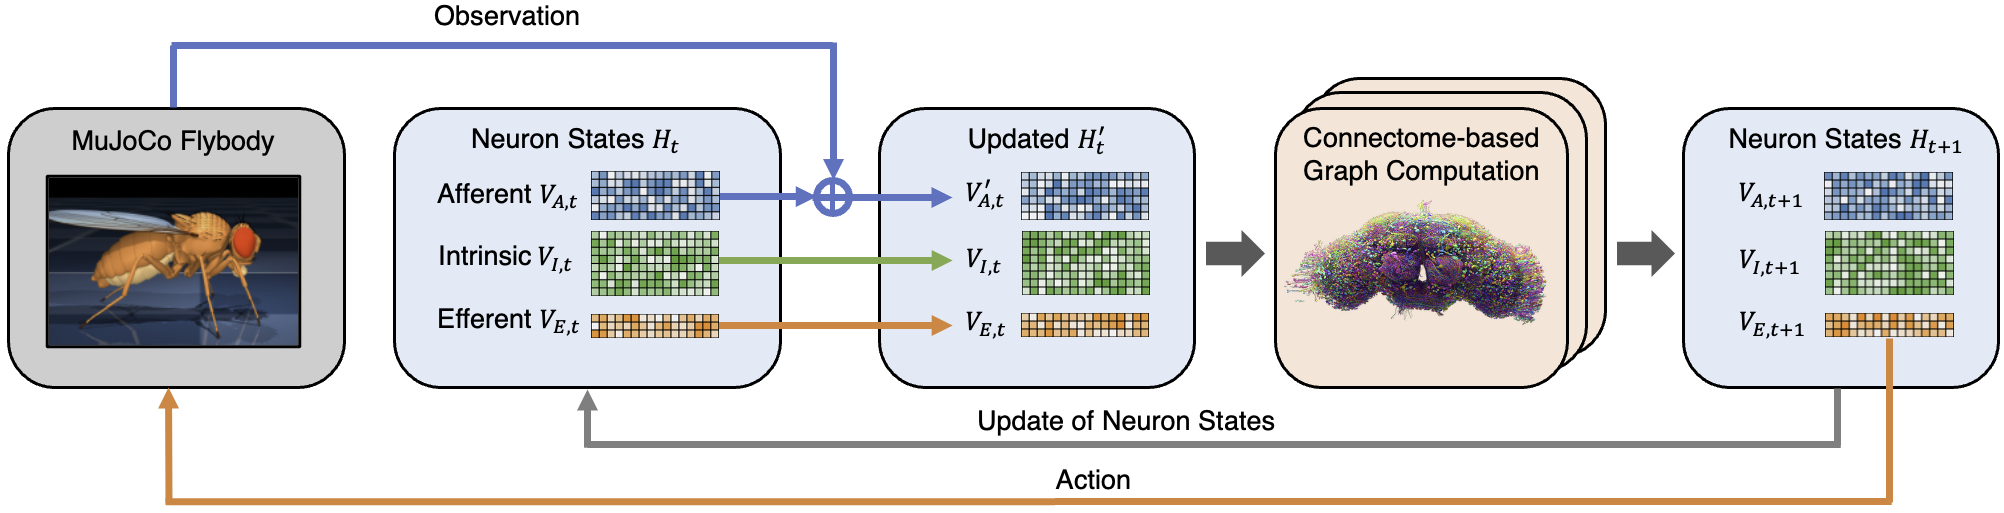
\includegraphics[width=0.9\linewidth]{figures/mainfig.png}
  \caption{\textbf{Overview of the FlyGM-enabled whole-body locomotion control framework.} Observations are mapped to afferent neuron states via a lightweight input projection. Neural states are propagated through a connectome-constrained message-passing module, and the resulting efferent states are decoded into motor actions that drive the embodied Drosophila model in MuJoCo. Demonstration videos and source code is available at: \url{https://lnsgroup.cc/research/FlyGM}.}
  \label{fig:mainfig}
\vskip -0.1in
\end{figure*}

Understanding the embodied learning of movement control is a long-standing challenge shared by artificial intelligence and neuroscience. Recent advances in neuroscience have revealed whole-brain connectomics in animals at synaptic resolution~\citep{Dorkenwald2024a}. These resources enable the possibility of linking complete brain structure to the sensorimotor control of a physical body. 

Advances in deep reinforcement learning present neural network controllers that can accomplish challenging movement tasks. However, these methods typically use hand-crafted networks (e.g. multilayer perceptrons). While effective for specific tasks, such neural architectures diverge significantly from biological circuits, limiting the interpretability of the learned computations and making it difficult to relate them to real nervous systems. Connectome-constrained models have provided insights into sensory and premotor computations~\citep{Azevedo2024}, yet most efforts remain limited to specific subsystems and simplified behaviors. Thus the fundamental challenge remains: how can static connectomes be transformed into dynamic, functional models that reproduce the intricate and adaptive motor behaviors of bodies? Answering this question requires bridging two active lines of research: (i) mechanistic modeling that leverages whole-brain connectivity, and (ii) learning frameworks that can control high-dimensional whole-body movements.

In this work, we develop the Fly-connectomic Graph Model (FlyGM), a neural controller whose computational architecture is directly inherited from the Drosophila whole-brain connectome. Without further neural architecture search or optimization, we use the connectome as a directed message-passing graph, partitioning nodes into afferent, intrinsic, and efferent sets to reflect biological information flow. By integrating this connectome-grounded policy with a physics-based fruit fly model, we demonstrate that the wiring of the fly brain provides a powerful structural inductive bias in embodied reinforcement learning.

Our experiments show that FlyGM achieves stable control across multiple locomotion tasks, including gait initiation, walking, turning, and flight. We verify the significance of this structural prior by comparing FlyGM against a degree-preserving rewired graph, a random graph, and multilayer perceptrons (MLP). Our results reveal that the new method yields significantly higher sample efficiency and lower error, suggesting that the connectome's organization is non-randomly optimized for the constraints of a physical body.

Beyond behavioral performance, we analyze the internal representations of FlyGM. We find that functional segregation across sensory, central, and motor populations emerges naturally from the trained dynamics. This differentiation occurs solely due to the structural constraints of the graph, providing evidence that biological wiring diagrams can induce functional specialization in artificial agents.

Our main contributions are summarized below:

\textbf{Connectome-Structured Architecture}: FlyGM is a graph neural controller instantiated from the whole-brain Drosophila connectome, transforming static biological wiring into a dynamic controller.

\textbf{Diverse Embodied Locomotion}: FlyGM enables whole-body biomechanical control across diverse tasks in high-fidelity physics simulations.

\textbf{Evidence of Structural Inductive Bias}: The biological connectome yields higher sample efficiency and performance compared to baseline models.

%\newpage
\section{Related Work}

\textbf{Connectomics-based neural network modeling.} Advances in connectomics have deepened our understanding of circuit-level organization in central nervous systems of animal models. In particular, the FlyWire project provides a whole-brain reconstruction of Drosophila at synaptic resolution, offering the structural basis for modeling complete neural dynamics~\citep{Dorkenwald2024a,Schlegel2024a,Zheng2018a}. Prior works have highlighted the explanatory power of such data in restricted domains: ventral nerve cord reconstructions revealed leg–wing coordination circuits~\citep{Azevedo2024,Lesser2024}, and models of motor neurons have been applied to feeding or grooming behaviors~\citep{Shiu2024}. Connectome-constrained networks have also been used to predict neural activity in the visual system~\citep{Lappalainen2024}. However, these approaches often focus on specific subsystems or tasks, leaving open the question whether whole-brain connectivity can generate realistic control of embodied locomotion behaviors.

\textbf{Embodied movement control.} In parallel, embodied intelligence research has advanced locomotion in simulated humanoids~\citep{Kumar2021,Cheng2024}, quadrupeds~\citep{Ding2021}, and musculoskeletal agents~\citep{he2024icml,Wei2025} using reinforcement learning. In the Drosophila domain, physics-based models such as NeuroMechFly~\citep{LobatoRios2022,WangChen2024} and flybody~\citep{Vaxenburg2025} have enabled detailed simulations of walking and flight in MuJoCo~\citep{todorov2012mujoco}. Yet, controllers for these systems are typically built from generic MLPs or manually designed central pattern generators, lacking direct biological grounding. This limits both interpretability and the ability to connect neural structure to behavior. Our work differs by directly embedding the connectome into the controller architecture, combining embodied simulation with structural priors to study both performance and neural representation.

\begin{figure*}[htbp]
  \centering
  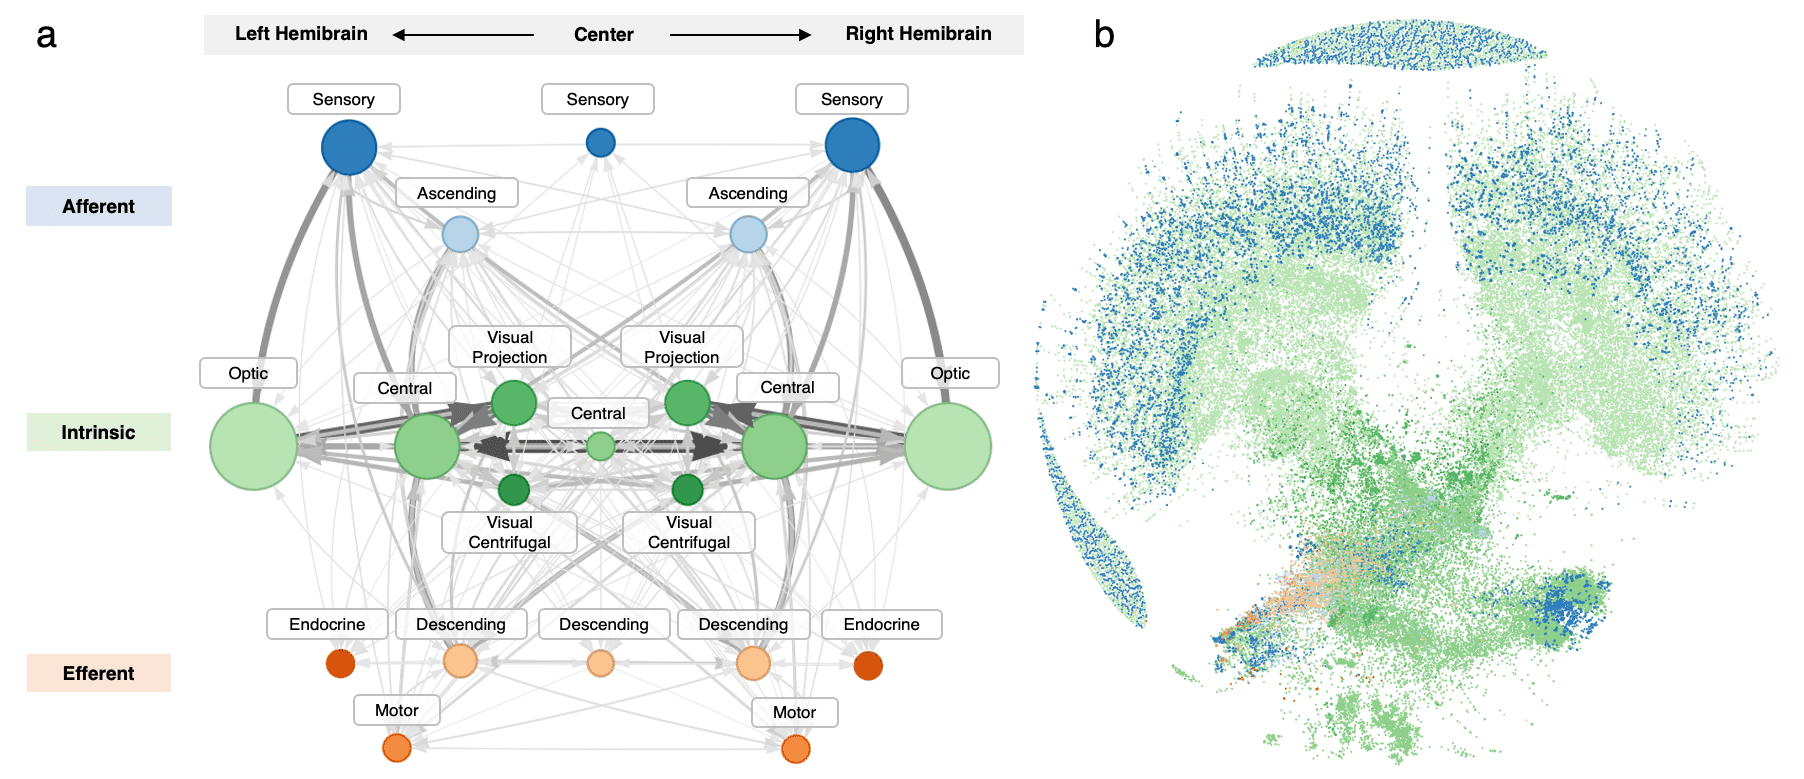
\includegraphics[width=0.9\textwidth]{figures/network.png}
  \caption{\textbf{Structure of the Fly-connectomic Graph.} \textbf{(a)} Aggregated synapse graph of the fly connectome, grouped into afferent (blue), intrinsic (green), and efferent (orange) sets across left hemibrain, central, and right hemibrain compartments. Node sizes reflect the number of neurons in each group, and arrows indicate the direction and relative strength of connectivity. \textbf{(b)} Force-directed graph layout~\citep{Kobourov2012} of the same neural network. The spatial layout reveals hemispheric symmetry and functional clustering.}
  \label{fig:connectome}
  \vskip -0.1in
\end{figure*}

\section{Method}
\label{sec:method}

\subsection{Connectome-structured Graph Model}

We consider the problem of embodied sensorimotor control for a virtual fruit fly agent interacting with a physics-based environment provided by flybody. Let the state at time step $t$ be denoted by $s_t \in \mathcal{S}$. The agent receives an observation $x_t \in \mathbb{R}^{d_{\text{in}}}$, which corresponds to a set of processed features including proprioceptive and exteroceptive signals during movement and environmental interaction. Based on this input, the neural controller produces an action $a_t \in \mathbb{R}^{d_{\text{out}}}$, representing motor outputs that drive the flybody model to perform locomotion behaviors.

We represent the Drosophila connectome as a directed synapse graph $G=(V,E)$, where nodes $V$ denote neurons and edges $E$ represent synaptic connections. Following the linear-dynamical connectome modeling perspective in ``effectome'' \citep{Pospisil2024}, the synaptic weight matrix $W \in \mathbb{R}^{|V| \times |V|}$ acts as a fixed, recurrent state-transition operator that dictates the information flow through the network.

To ground the model's latent dynamics in biological reality, we refine the synaptic weights by incorporating the functional polarity of presynaptic neurons. Based on established Drosophila cell type annotations, we categorize major neurotransmitters into two functional sets:
\vspace{-0.5em}
\begin{itemize}
    \setlength{\itemsep}{0pt}
    \item \textbf{Excitatory ($\mathcal{S}_{\text{exc}}$):} Acetylcholine (ACH), Glutamate (GLU), Aspartate (ASP), and Histamine (HIS).
    \item \textbf{Inhibitory ($\mathcal{S}_{\text{inh}}$):} $\gamma$-aminobutyric acid (GABA) and Glycine (GLY).
\end{itemize}
\vspace{-0.5em}

Following this categorization, the signed strength $W_{vu}$ for a directed edge from neuron $u$ to $v$ is defined as the net polarized synaptic count:
\begin{equation}
    W_{vu} = N_{\text{exc}}(u, v) - N_{\text{inh}}(u, v)
\end{equation}
where $N_{\text{exc}}$ and $N_{\text{inh}}$ are the total synapse counts associated with excitatory and inhibitory neurotransmitters, respectively. This signed weighting scheme ensures that the message-passing operation $M_t = W H_t$ respects the sign-preserving or sign-reversing nature of biological signal propagation, consistent with the methodology proposed by \citet{Pospisil2024}.

Following FlyWire’s classification of flow types, we partition neurons into three disjoint sets:
\vspace{-0.5em}
\begin{itemize}
\setlength{\itemsep}{0pt}
\setlength{\parsep}{0pt}
\setlength{\parskip}{0pt}
\item \textbf{Afferent neurons}: $V_a \subset V$, which receive external sensory inputs,
\item \textbf{Intrinsic neurons}: $V_i \subset V$, which mediate signals within the network, and
\item \textbf{Efferent neurons}: $V_e \subset V$, which produce motor outputs to the body model.
\end{itemize}
\vspace{-0.5em}

Thus, $V = V_a \cup V_i \cup V_e$ with $V_a \cap V_i \cap V_e = \emptyset$. Each neuron $v \in V$ is associated with a latent state vector $h_{v,t} \in \mathbb{R}^{C}$, and we collect all neuron states at time $t$ as a matrix:
\begin{equation}
H_t = \begin{bmatrix} h_{1,t}^\top \\ \vdots \\ h_{|V|,t}^\top \end{bmatrix} \in \mathbb{R}^{|V| \times C}.
\end{equation}

Beyond the shared synaptic operator $W$, we assign each neuron a trainable intrinsic descriptor $\eta_v \in \mathbb{R}^{D}$ to capture cell-specific computational properties (e.g., excitability and gain) that are not included in the connectomic data. The matrix stacking all intrinsic descriptors is represented as $\eta \in \mathbb{R}^{|V|\times D}$.

At each time step, sensory observation $x_t$ is first encoded by an encoder $\mathrm{Enc}_\theta$ and injected into afferent neurons via a gating map:
\begin{align}
\tilde{x}_t &= \mathrm{Enc}_\theta(x_t) \in \mathbb{R}^{d_{\text{enc}}},\\
H_t[V_a] &\leftarrow \tanh\!\big(W_g\,[\,H_t[V_a] \,\Vert\, \mathbf{1}\tilde{x}_t^\top\,] + b_g\big),
\end{align}
where $\mathbf{1}\tilde{x}_t^\top$ propagates the encoded observation to all afferent neurons. The encoder $\mathrm{Enc}_\theta$ compresses the high-dimensional observation $x_t$ into a low-dimensional representation (e.g., $d_{\text{enc}}=32$) before projecting to $V_a$, avoiding expensive per-neuron encoding and allowing the connectome-conditioned recurrent dynamics to carry out most of the computation.

Given the current network state $H_t$, we compute synaptic aggregation by applying connectome-derived synaptic weights as a linear operator:
\begin{equation}
M_t = W H_t \in \mathbb{R}^{|V|\times C},
\end{equation}
so that each neuron receives the weighted sum of its presynaptic partners’ states.

We then update each neuron state through a shared MLP $f_\psi$ conditioned on the neuron’s intrinsic descriptor:
\begin{equation}
H_{t+1}[v] = f_\psi\big(\,[\,M_t[v] \,\Vert\, \eta_v\,] \,\big), \quad v\in V.
\end{equation}
Equivalently, this can be viewed as a conditional state transition $p(H_{t+1} \mid M_t, \eta)$ where $M_t$ provides the synaptically aggregated evidence and $\eta$ supplies neuron-specific conditions that modulate how the evidence updates the state. In this sense, the connectome defines the topology and strength of information flow, while per-neuron trainable parameters determine how each neuron transforms and gates the incoming synaptic drive.

The updated efferent states $H_{t+1}[V_e]$ are flattened and mapped to continuous motor actions by a decoder $\mathrm{Dec}_\phi$:
\begin{equation}
a_t = \mathrm{Dec}_\phi\!\big(H_{t+1}[V_e]\big).
\end{equation}

The output actions serve as motor commands to actuate the flybody, a biomechanical model of the fruit fly implemented in MuJoCo~\citep{Vaxenburg2025}. Subsequent observation $x_{t+1}$ is then generated to close the sensorimotor loop.

In summary, Algorithm~\ref{alg:FlyGM } outlines the forward computation of FlyGM: observation injection into afferent neurons, synapse-weighted aggregation via the connectome operator, neuron-wise conditional updates using intrinsic descriptors, and efferent decoding into motor actions.

\begin{algorithm}[tb]
  \caption{Fly-connectomic Graph Model (FlyGM)}
  \label{alg:FlyGM }
  \begin{algorithmic}[1]
    \STATE {\bfseries Input:} Sensory input $x_t$; connectome $G=(V,E)$ with synapse weight matrix $W$; node partitions $V_a, V_i, V_e$;
    encoder $\mathrm{Enc_\theta}$; afferent gate $(W_g,b_g)$; neuron intrinsic descriptors $\{\eta_v\}_{v\in V}$;
    conditional update MLP $f_\psi$; decoder $\mathrm{Dec_\phi}$
    \STATE {\bfseries Output:} Motor output $a_t$

    \FOR{each time step $t$}
      \STATE $\tilde{x}_t \gets \mathrm{Enc_\theta}(x_t)$
      \STATE $H_t[V_a] \gets \tanh\!\big(W_g [H_t[V_a], \mathbf{1}\tilde{x}_t^\top] + b_g\big)$
      \STATE $M_t \gets W H_t$
      \STATE $H_{t+1}[v] \gets f_\psi([M_t[v], \eta_v]) \quad \forall v\in V$
      \STATE $a_t \gets \mathrm{Dec_\phi}(H_{t+1}[V_e])$
      \STATE Apply $a_t$ to Flybody in MuJoCo to obtain $x_{t+1}$
    \ENDFOR
  \end{algorithmic}
\end{algorithm}

\subsection{Training Pipeline}

Our training pipeline consisted of two stages: first, we initialized the connectome-based policy using imitation learning from expert trajectories, and secondly we fine-tuned the model with reinforcement learning to directly optimize for task rewards. This two-stage design leveraged demonstration data for rapid initialization while preserving the capability for adaptive policy improvement.

To provide an initial policy, we collected expert trajectories by rolling out an MLP-based policy for the flybody which was originally trained with imitation learning to generate high-quality demonstrations of locomotion. We used these trajectories to train our connectome-based model by imitating the expert’s action distributions. 

Specifically, the policy predicted Gaussian parameters $(\mu_s, \sigma_s)$ given the same observations as the expert, and was optimized to minimize a loss combining Kullback–Leibler divergence with an annealed mean squared error (MSE) regularizer:
\begin{equation}
\begin{aligned}
    \mathcal{L}_t &= D_{\mathrm{KL}}\!\left( \mathcal{N}(\mu_t, \sigma_t^2) \;\|\; \mathcal{N}(\mu_s, \sigma_s^2) \right) \\
    &\quad + \lambda(t) \Big( \|\mu_s - \mu_t\|_2^2 + \alpha \,\|\log \sigma_s - \log \sigma_t\|_2^2 \Big)
\end{aligned}
\end{equation}

where $\alpha$ is a constant to balance the scale of $\mu_s$ and $\log \sigma_s$, and $\lambda(t)$ decreases during training so that distributional matching dominates in later stages. This procedure initialized the model with stable behaviors for walking and flight tasks.


After initialization, we fine-tuned the connectome-structured policy using Proximal Policy Optimization (PPO) to enable direct learning from rewards. For value estimation, we used a simple MLP as the value network. The environments in MuJoCo were adapted into gym-like interfaces with parallel rollouts to increase throughput, and distributed training with Distributed Data Parallel (DDP) was used for scalability. The policy was updated following the clipped surrogate objective with value and entropy regularization:
\begin{equation}
\begin{aligned}
\mathcal{L}_{\text{PPO}} &= \mathbb{E}_t \Big[ \min\big(r_t(\theta) \hat{A}_t, \text{clip}(r_t(\theta), 1-\epsilon, 1+\epsilon)\hat{A}_t\big) \\
&\quad - c_v (V_\theta(s_t) - R_t)^2 + c_e \mathcal{H}[\pi_\theta(\cdot|s_t)] \Big]
\end{aligned}
\end{equation}
where $ r_t(\theta)=\frac{\pi_\theta(a_t \mid s_t)}{\pi_{\theta_{\text{old}}}(a_t \mid s_t)} $ is the probability ratio between new and old policies, $\hat{A}_t$ is the GAE advantage, $R_t$ is the return, and $\mathcal{H}$ is the entropy bonus. This stage allowed the model to improve beyond demonstration data and adapt to task-specific dynamics while retaining the inductive bias imposed by the connectome architecture.


\section{Experiments}

We evaluated FlyGM on four locomotor tasks with the flybody physics simulator~\citep{Vaxenburg2025}, comprising three terrestrial tasks (gait initiation, straight walking, and turning) and one flight task. These tasks are categorized into two primary behavioral domains (walking and flying) for which flybody provided distinct pre-trained MLP controllers and real-world Drosophila motion capture datasets. We followed the default flybody environment setup and added binocular visual signals to the original sensory inputs for walking tasks to provide multimodal feedback (proprioception, mechanosensation, and vision).

To support the imitation learning stage, we constructed a domain-specific behavioral dataset by performing rollouts of the corresponding pretrained models across their respective biological trajectories. We filtered these rollouts to include only successful episodes exceeding 100 steps, resulting in a comprehensive dataset of synchronized observation-action time series. This curated dataset captures the high-fidelity, naturalistic motor patterns necessary to test whether a connectome-structured network can flexibly generate stable control policies across distinct movement modes.

Detailed training procedures and hyperparameters are provided in Appendix~\ref{app:train_details}, and observation/action definitions are provided in Appendix~\ref{app:env_details}. Demonstration videos for each task are available on our project webpage.

\subsection{Inductive Bias from Connectome Topology}
\label{sec:inductive_bias}

\begin{table*}[t]
\centering
\small
\begin{tabular}{lcccc}
\toprule
\textbf{Model} & \textbf{speed=2, yaw=0} & \textbf{speed=3, yaw=0} & \textbf{speed=3, yaw=4} & \textbf{speed=3, yaw=7} \\
\midrule
\textbf{Connectome-Based FlyGM} & & & & \\
\quad Pos Err $\downarrow$ & $0.0280\pm0.001$ & \boldmath$0.0364\pm0.001$ & $0.0327\pm0.001$ & \boldmath$0.0364\pm0.002$ \\
\quad Angle Err $\downarrow$ & \boldmath$4.96\pm0.09$ & \boldmath$5.57\pm0.06$ & \boldmath$6.36\pm0.33$ & \boldmath$8.29\pm0.21$ \\
\midrule
\textbf{Degree-Preserving Rewiring Graph} & & & & \\
\quad Pos Err $\downarrow$ & \boldmath$0.0272\pm0.001$ & $0.0385\pm0.000$ & \boldmath$0.0310\pm0.000$ & $0.0370\pm0.002$ \\
\quad Angle Err $\downarrow$ & $7.84\pm0.08$ & $7.77\pm0.08$ & $9.72\pm0.12$ & $13.55\pm0.69$ \\
\midrule
\textbf{Erd\H{o}s--R\'enyi Random Graph} & & & & \\
\quad Pos Err $\downarrow$ & $0.0449\pm0.002$ & $0.0485\pm0.001$ & $0.0562\pm0.001$ & $0.6278\pm0.040$ \\
\quad Angle Err $\downarrow$ & $12.11\pm0.23$ & $11.33\pm0.27$ & $17.45\pm0.26$ & $125.36\pm8.96$ \\
\bottomrule
\end{tabular}
\caption{Comparison of different graph topologies across varying speed and yaw conditions. Values are reported as mean$\pm$std. Bold values indicate the best performance (minimum error) in each category.}
\label{tab:topology_reduction}
\vskip -0.1in
\end{table*}

To evaluate whether the biological connectome provides a structural inductive bias beyond mere parameter count, we compared the \textbf{Connectome} topology against three distinct baselines while maintaining an identical reinforcement learning pipeline. We first considered two graph-based variants: (i) an \textbf{Erd\H{o}s--R\'enyi random graph} with the same number of nodes and edges as the biological connectome, and (ii) a \textbf{degree-preserving rewiring graph} generated by randomly shuffling the edges of the connectome while strictly maintaining the in-degree and out-degree of each individual neuron. Additionally, we implemented a \textbf{MLP} baseline that retains the same input encoder but replaces the connectome-conditioned graph computation with a standard feed-forward architecture. By comparing the performance of the biological connectome against these non-connectome models, we could isolate the specific contribution of the evolved brain wiring to the efficiency and stability of embodied locomotion control.

In our experimental setup for the graph-based non-connectome models, all edges were treated as unweighted with unit strength. This assumption was reasonable since the integrity was preserved through trainable intrinsic node descriptors, and the injective sum aggregation was sufficient to capture structural properties without additional weighting~\citep{Xu2019}.

To ensure a rigorous comparison, we set a consistent dimensionality of 32 for all components, including the encoder output dimension, the latent channel dimension $C$, and the intrinsic descriptor dimension $D$. For the MLP baseline, the model followed the same encoder but replaced the graph computation with two fully-connected layers, each with a hidden dimension of 512. 

\begin{figure}[h]
  \centering
  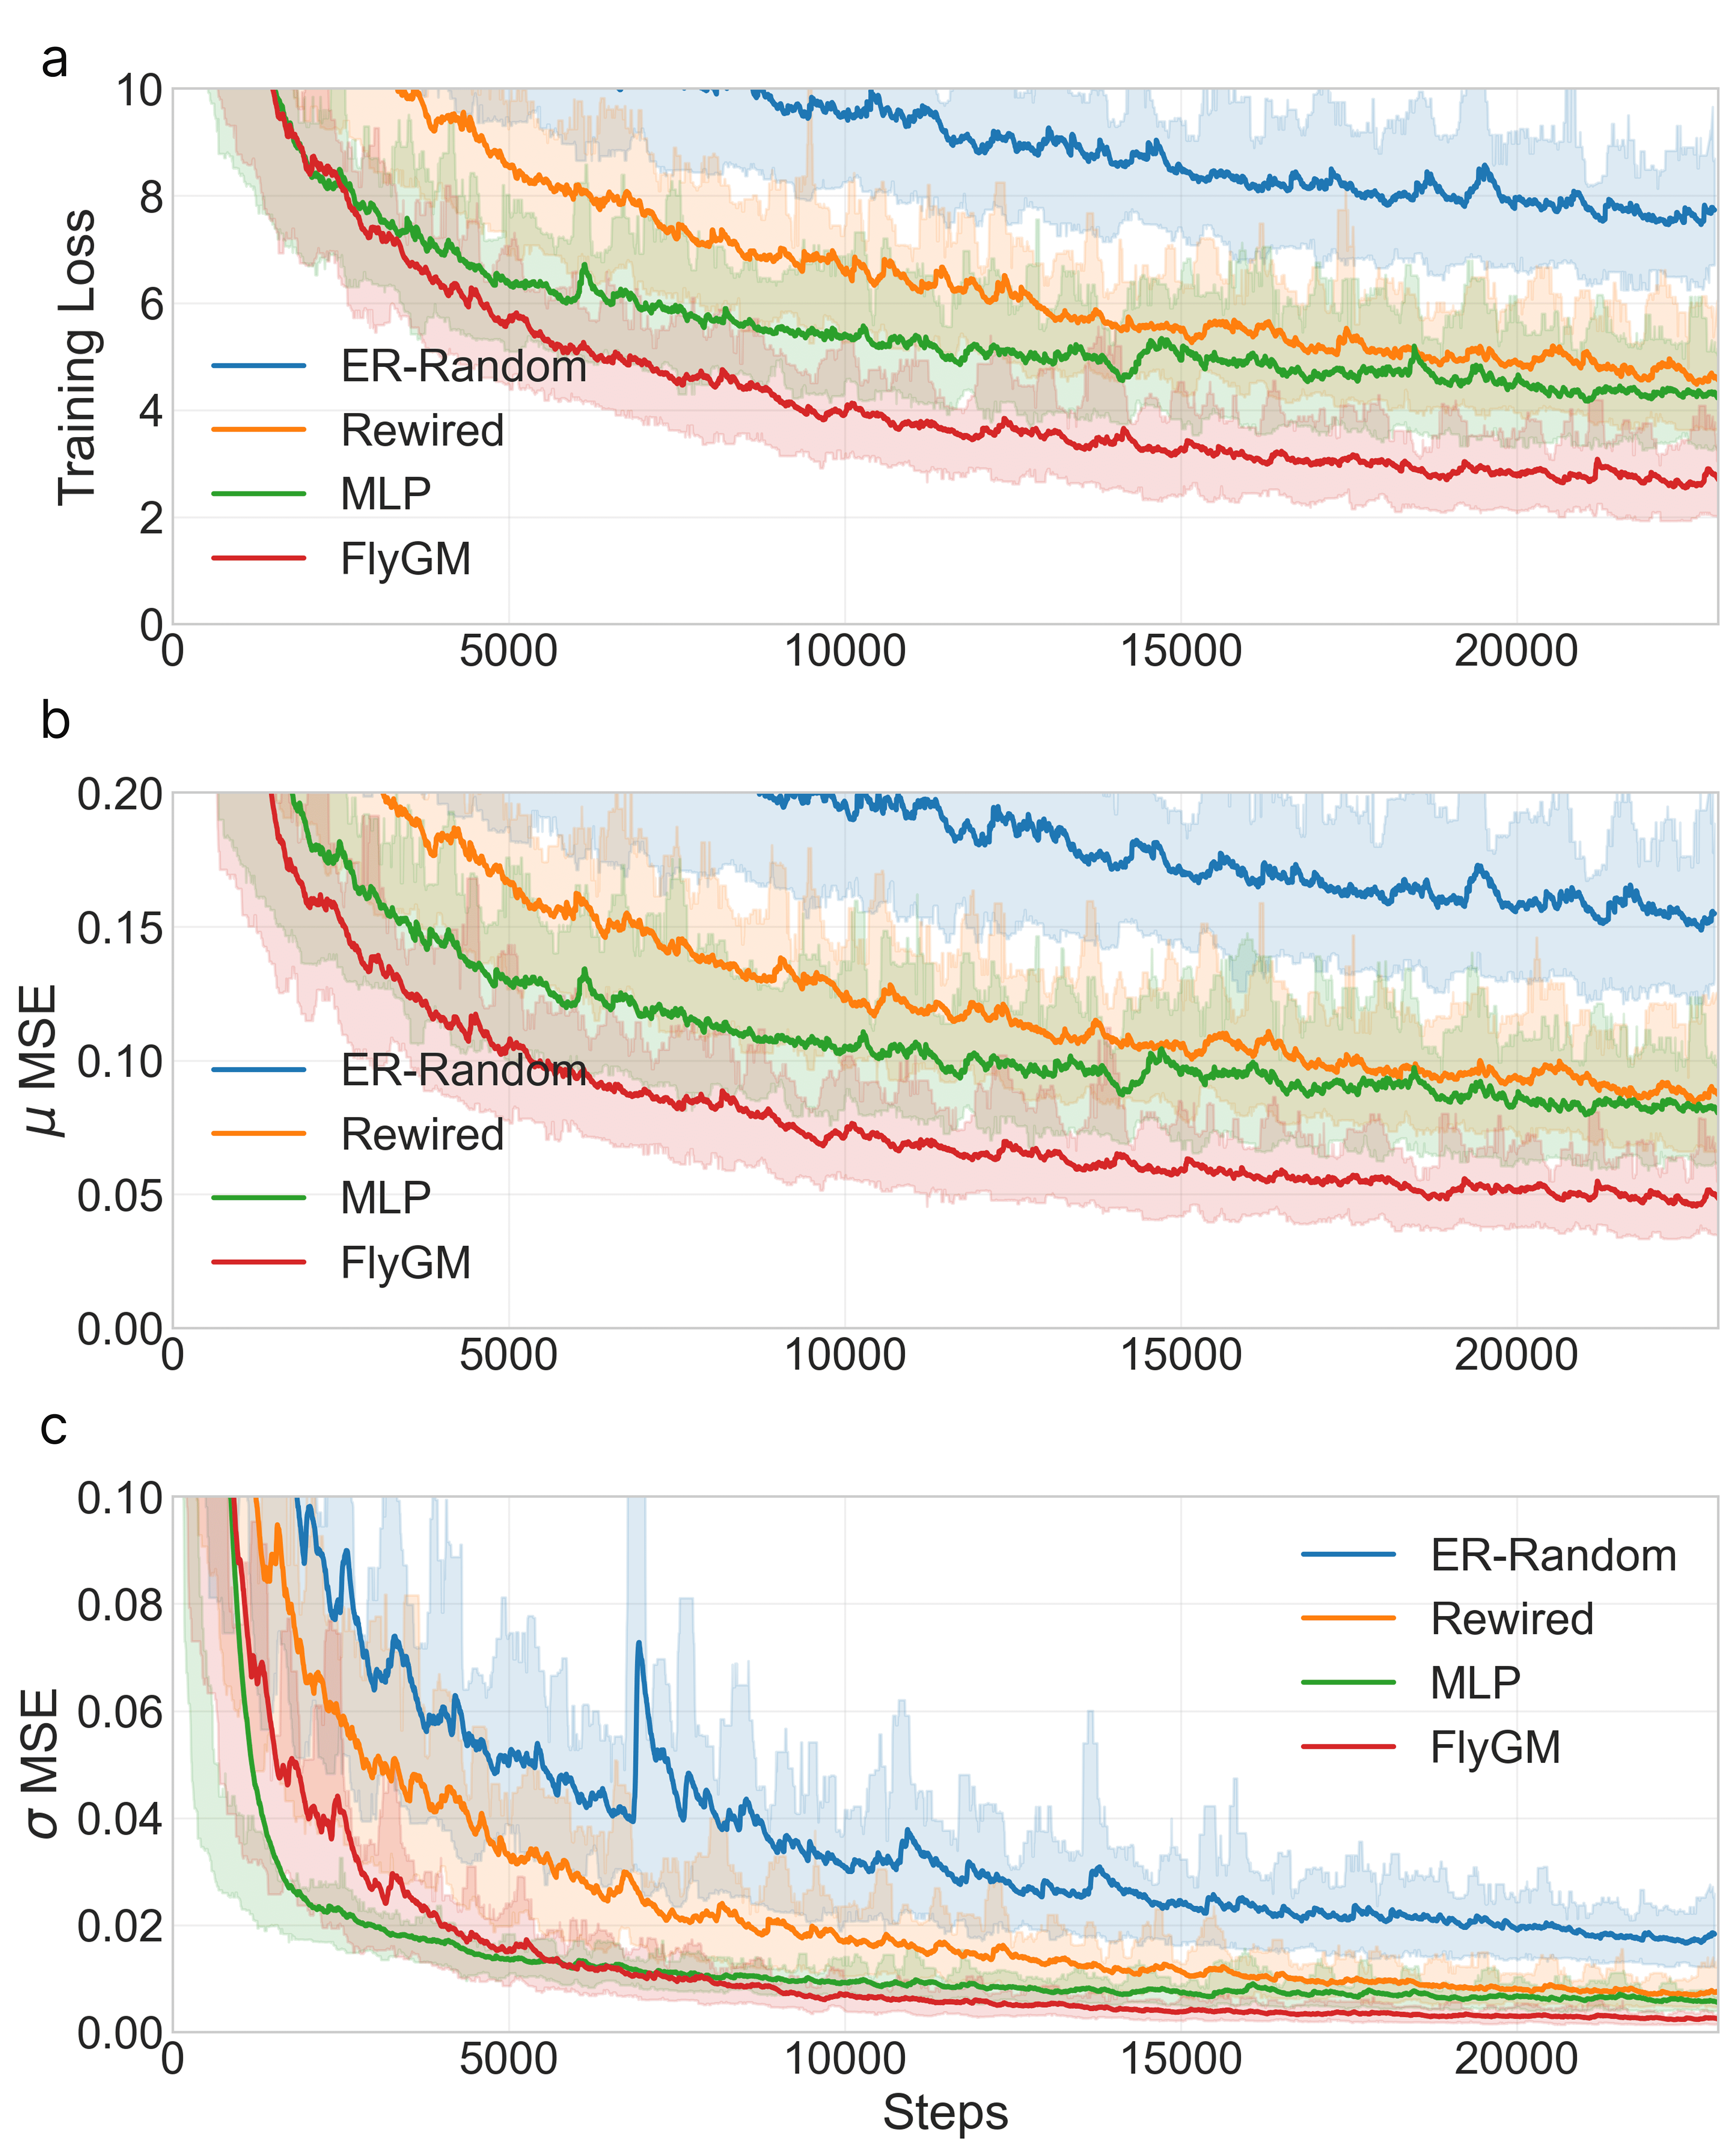
\includegraphics[width=0.48\textwidth]{figures/bias.png}
    \caption{Learning efficiency and metrics across different graph topologies and architectures. (a) Total training loss; (b) mean squared error of action means ($\mu$ MSE), and (c) mean squared error of action log-standard deviations ($\sigma$ MSE) during the imitation learning stage. Shaded areas represent the standard deviation across multiple training runs. ER-Random: Erd\H{o}s--R\'enyi random graph; Rewired: degree-preserving rewired graph; MLP: multilayer perceptron.}
  \label{fig:bias}
\end{figure}

We focused our evaluation on the imitation learning stage, which provided a stable environment to assess the structural advantages of the network from scratch. As illustrated in Figure~\ref{fig:bias}, we compare the training dynamics across three key metrics: (1) Total training loss (Fig.~\ref{fig:bias}a), which serves as a proxy for sample efficiency; and the Mean Squared Error (MSE) of the action (2) means ($\mu$, Fig.~\ref{fig:bias}b) and (3) standard deviations ($\sigma$, Fig.~\ref{fig:bias}c) relative to the expert trajectories, reflecting the fidelity of trajectory tracking.

Our results demonstrate that the biological connectome-based architecture consistently outperforms all other graph topologies across all metrics. Notably, the connectome exhibits a markedly superior sample efficiency, converging faster and getting lower MSE than the non-connectome models. This performance gap suggests that the specific wiring of the fruit fly brain provides a meaningful inductive bias tailored for embodied locomotion.

Table~\ref{tab:topology_reduction} quantifies the control performance across varying command configurations, with linear speed measured in cm/s and yaw rate in rad/s. As task complexity increases, the structural advantages of the biological connectome become increasingly apparent. While the Degree-Preserving Rewiring Graph remains competitive in terms of position error, it fails to maintain angular stability, incurring significantly higher angle errors than the connectome in all scenarios. This disparity is most pronounced in the high-yaw condition, where the Connectome-Based FlyGM maintains an angle error of 8.29 rad/s, whereas the rewired model degrades to 13.55 rad/s. The Erd\H{o}s--R'enyi Random Graph collapses under these complex conditions, exhibiting a catastrophic angle error of 125.36 rad/s. These results suggest that the wiring specificity of the biological connectome are essential for stable, high-fidelity orientation control during complex maneuvers.

\subsection{Performance on Locomotion Tasks}

\textbf{Gait Initiation}

Building on the training pipeline described above, we evaluated FlyGM on a walking task at a target velocity of 3 cm/s. We first examined the process of gait initiation, focusing on the transition from rest to the onset of stable locomotion. Figure~\ref{fig:flystart} illustrates snapshots of the simulated fly prior to the first complete gait cycle. It successfully initiated the movement in roughly the first 80 ms, during which irregular steps gradually gave way to rhythmic and coordinated leg movements.
\label{sec:walk_task}

\begin{figure}[htbp]
  \centering
  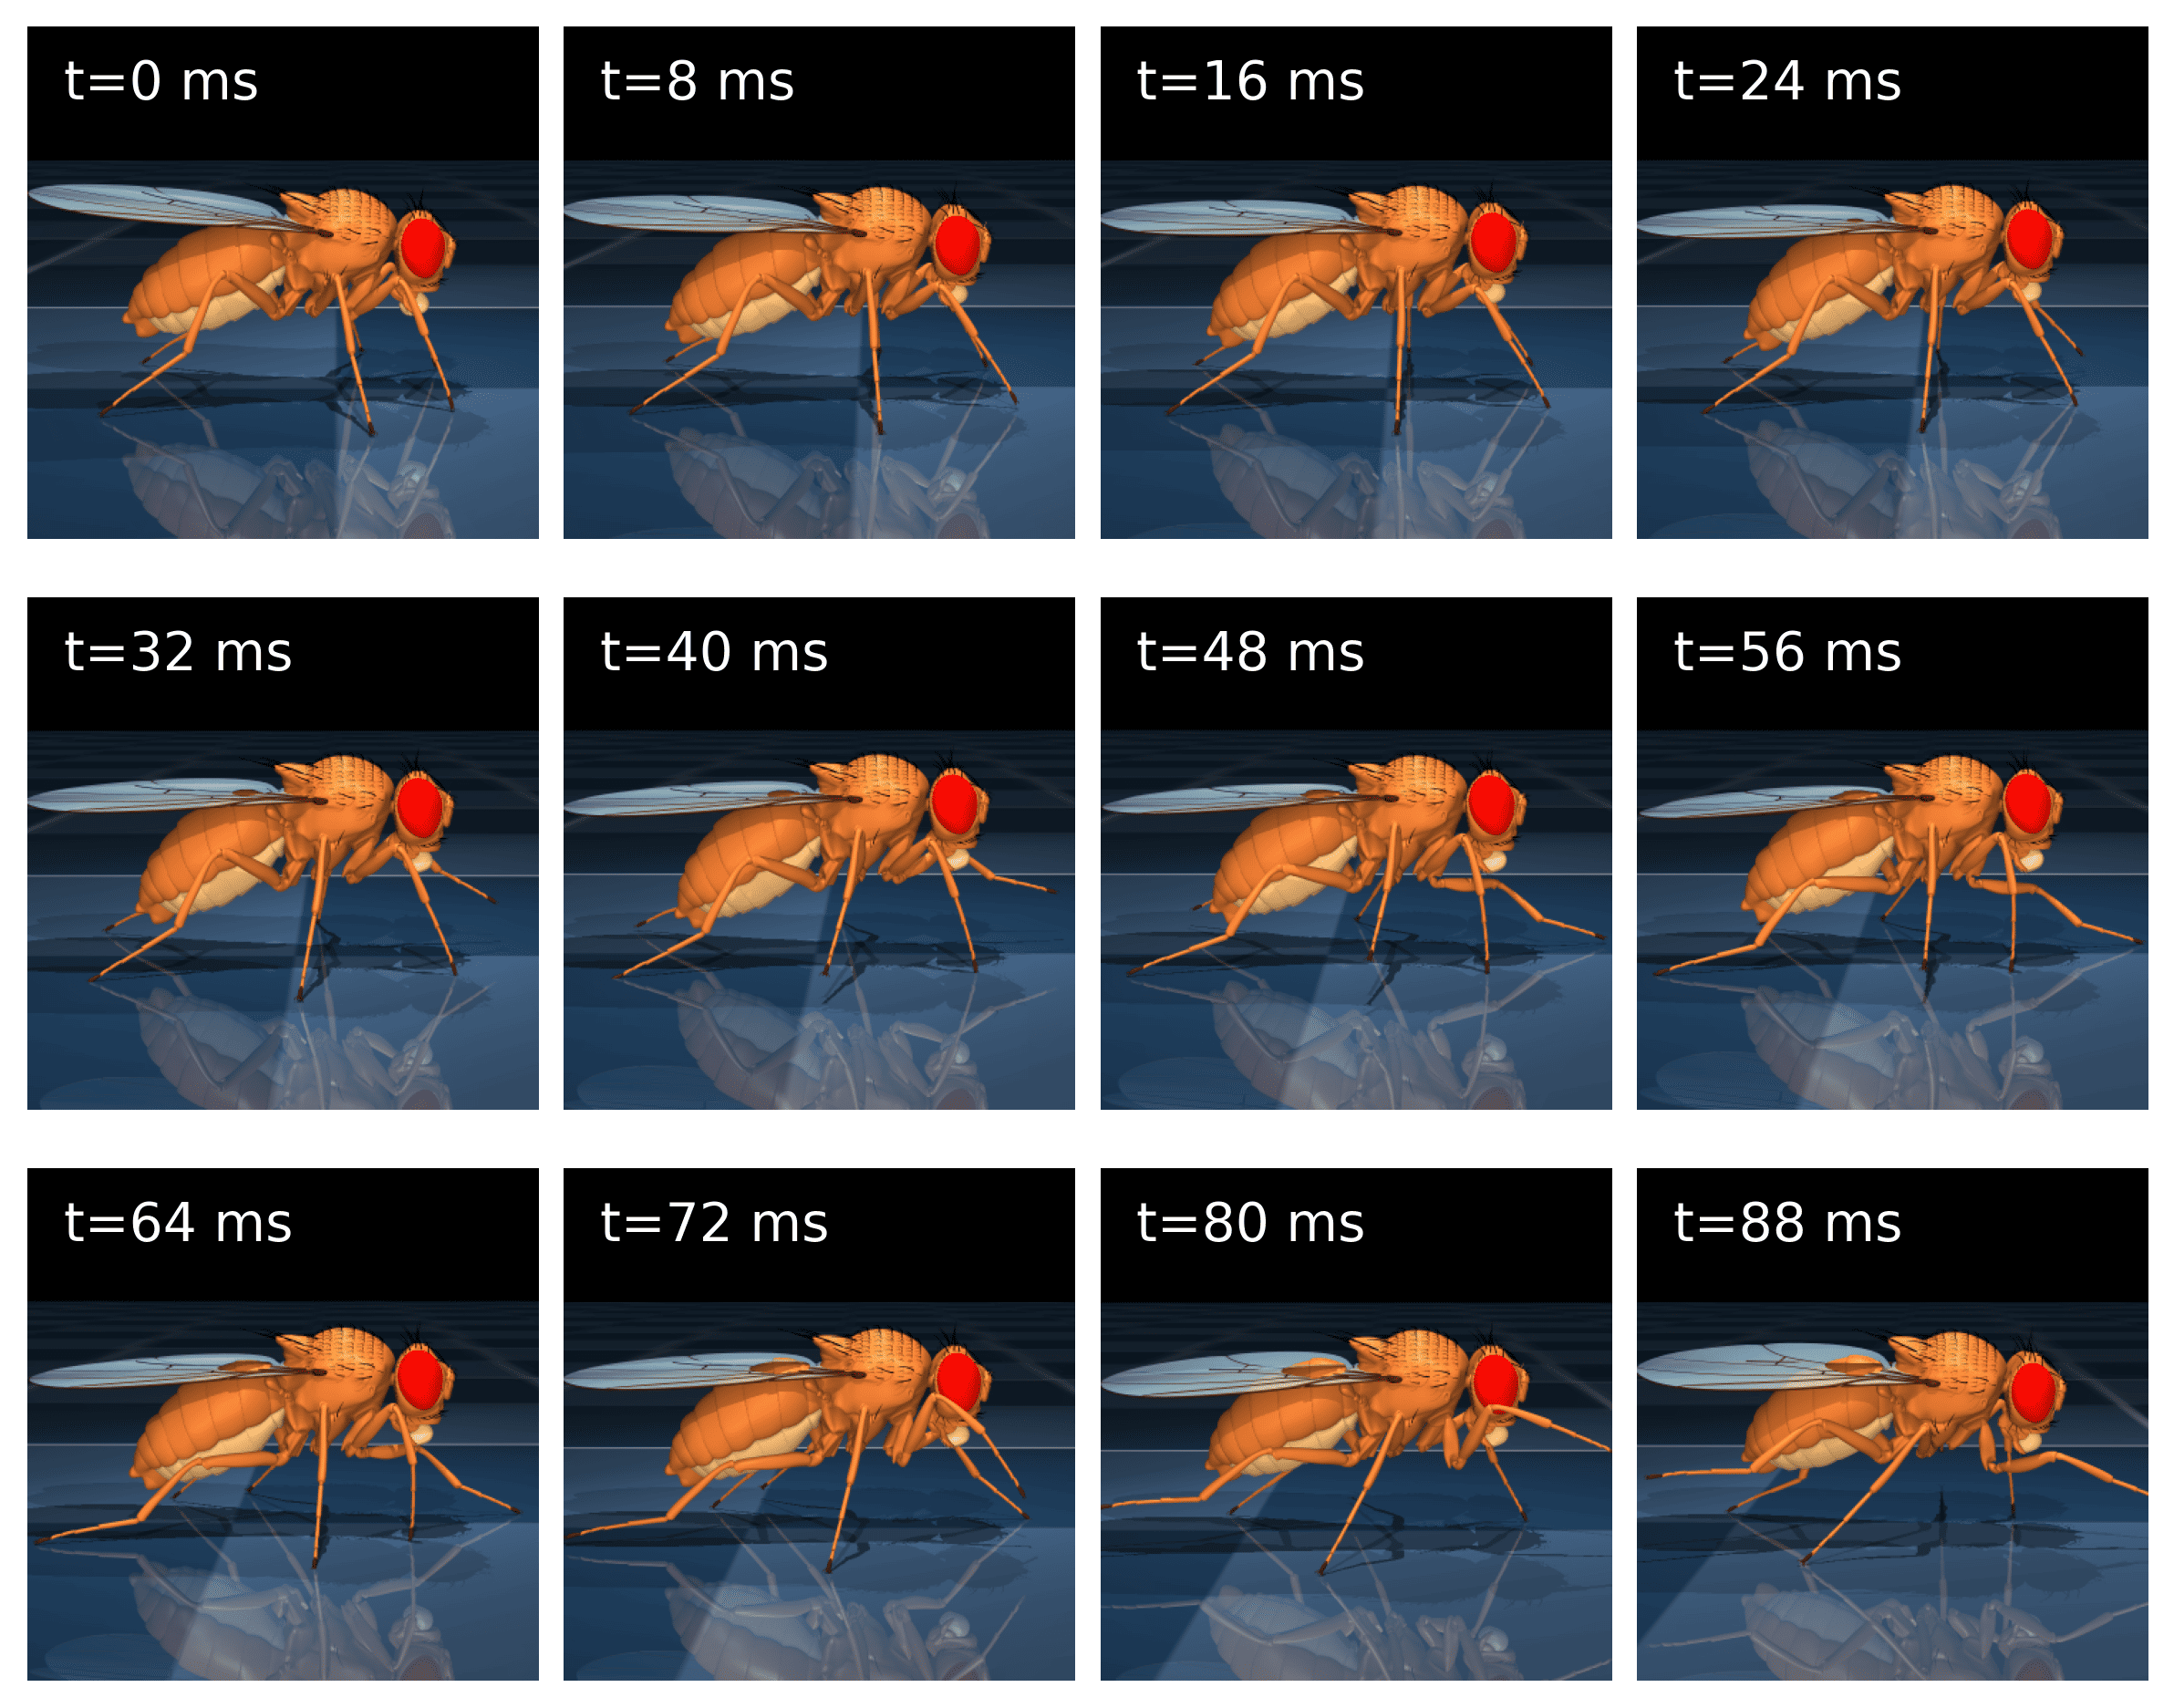
\includegraphics[width=0.395\textwidth]{figures/flystart.png}
  \caption{\textbf{Gait initiation dynamics.} 
  Snapshots of the simulated fly during the gait initialization phase.}
  \label{fig:flystart}
\end{figure}

\textbf{Straight-Line Walking}

Following the analysis of gait initiation, we next evaluated FlyGM on the straight-line walking phase at a target velocity of 3 cm/s. As illustrated in Figure \ref{fig:flywalk}, the flybody model performed stable forward locomotion with clear tripod coordination. The simulated fly maintained a consistent body trajectory over hundreds of milliseconds without drift or collapse, indicating that the learned controller generalized well to continuous walking.

Joint-level analysis (See Appendix~\ref{app:kinematics} for quantitative results) in Figure \ref{fig:coxa} shows that actuator outputs are tightly coupled with kinematic trajectories: contralateral legs alternate in phase, producing the classical tripod gait pattern seen in Drosophila. These results demonstrate that FlyGM is sufficient to generate stable straight walking once locomotion is initiated.

\begin{figure}[htbp]
  \centering
  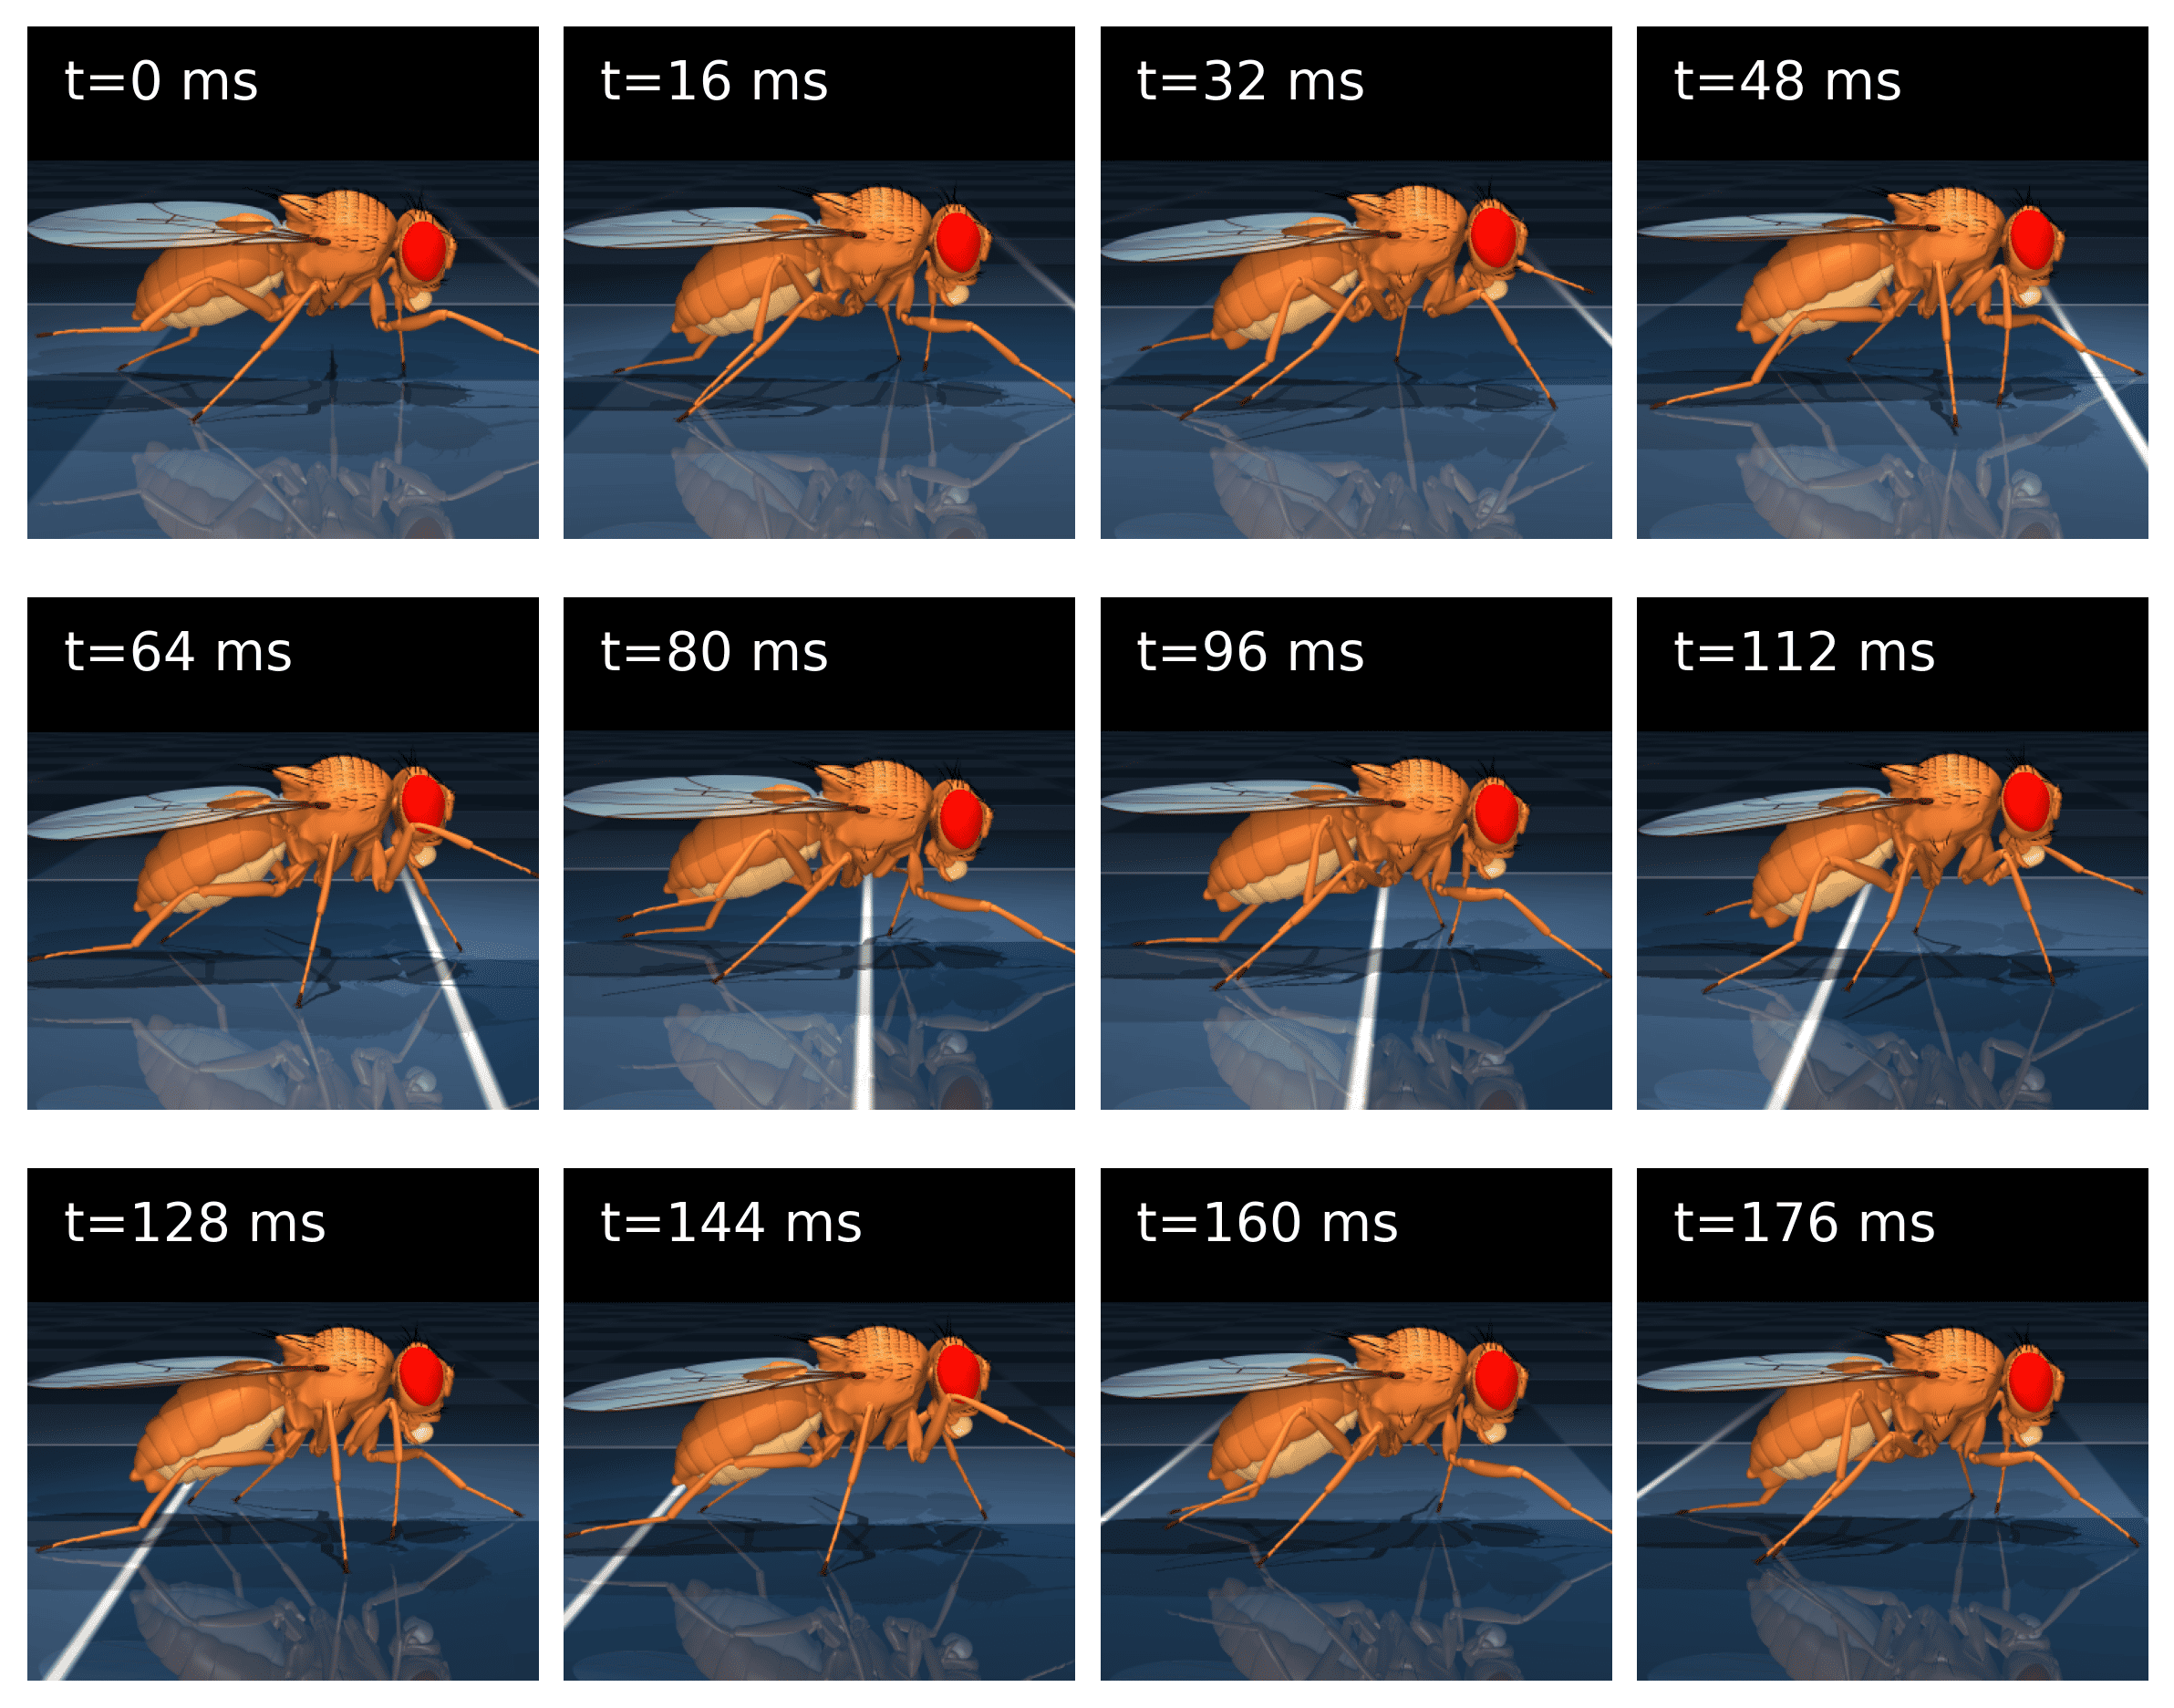
\includegraphics[width=0.395\textwidth]{figures/flywalk.png}
  \caption{\textbf{Walking dynamics.} 
  Snapshots of the simulated fly walking in a straight line at a velocity of 3 cm/s. }
  \label{fig:flywalk}
\end{figure}

\textbf{Turning}

\label{sec:turn_task}

We next assessed whether the same policy could generalize to directional maneuvers. In the turning task, the model was instructed to walk at a forward velocity of 3 cm/s while executing a leftward turn at 10 rad/s. As shown in Figure \ref{fig:flyturn}, the simulated fly successfully produced a smooth curved trajectory by modulating stride lengths asymmetrically across the body: legs on the inner side of the turn reduced their stance amplitude, while contralateral legs extended their strides. This modulation of gait symmetry arised naturally from the network dynamics, without requiring task-specific tuning or additional control rules.
\begin{figure}[htbp]
  \centering
  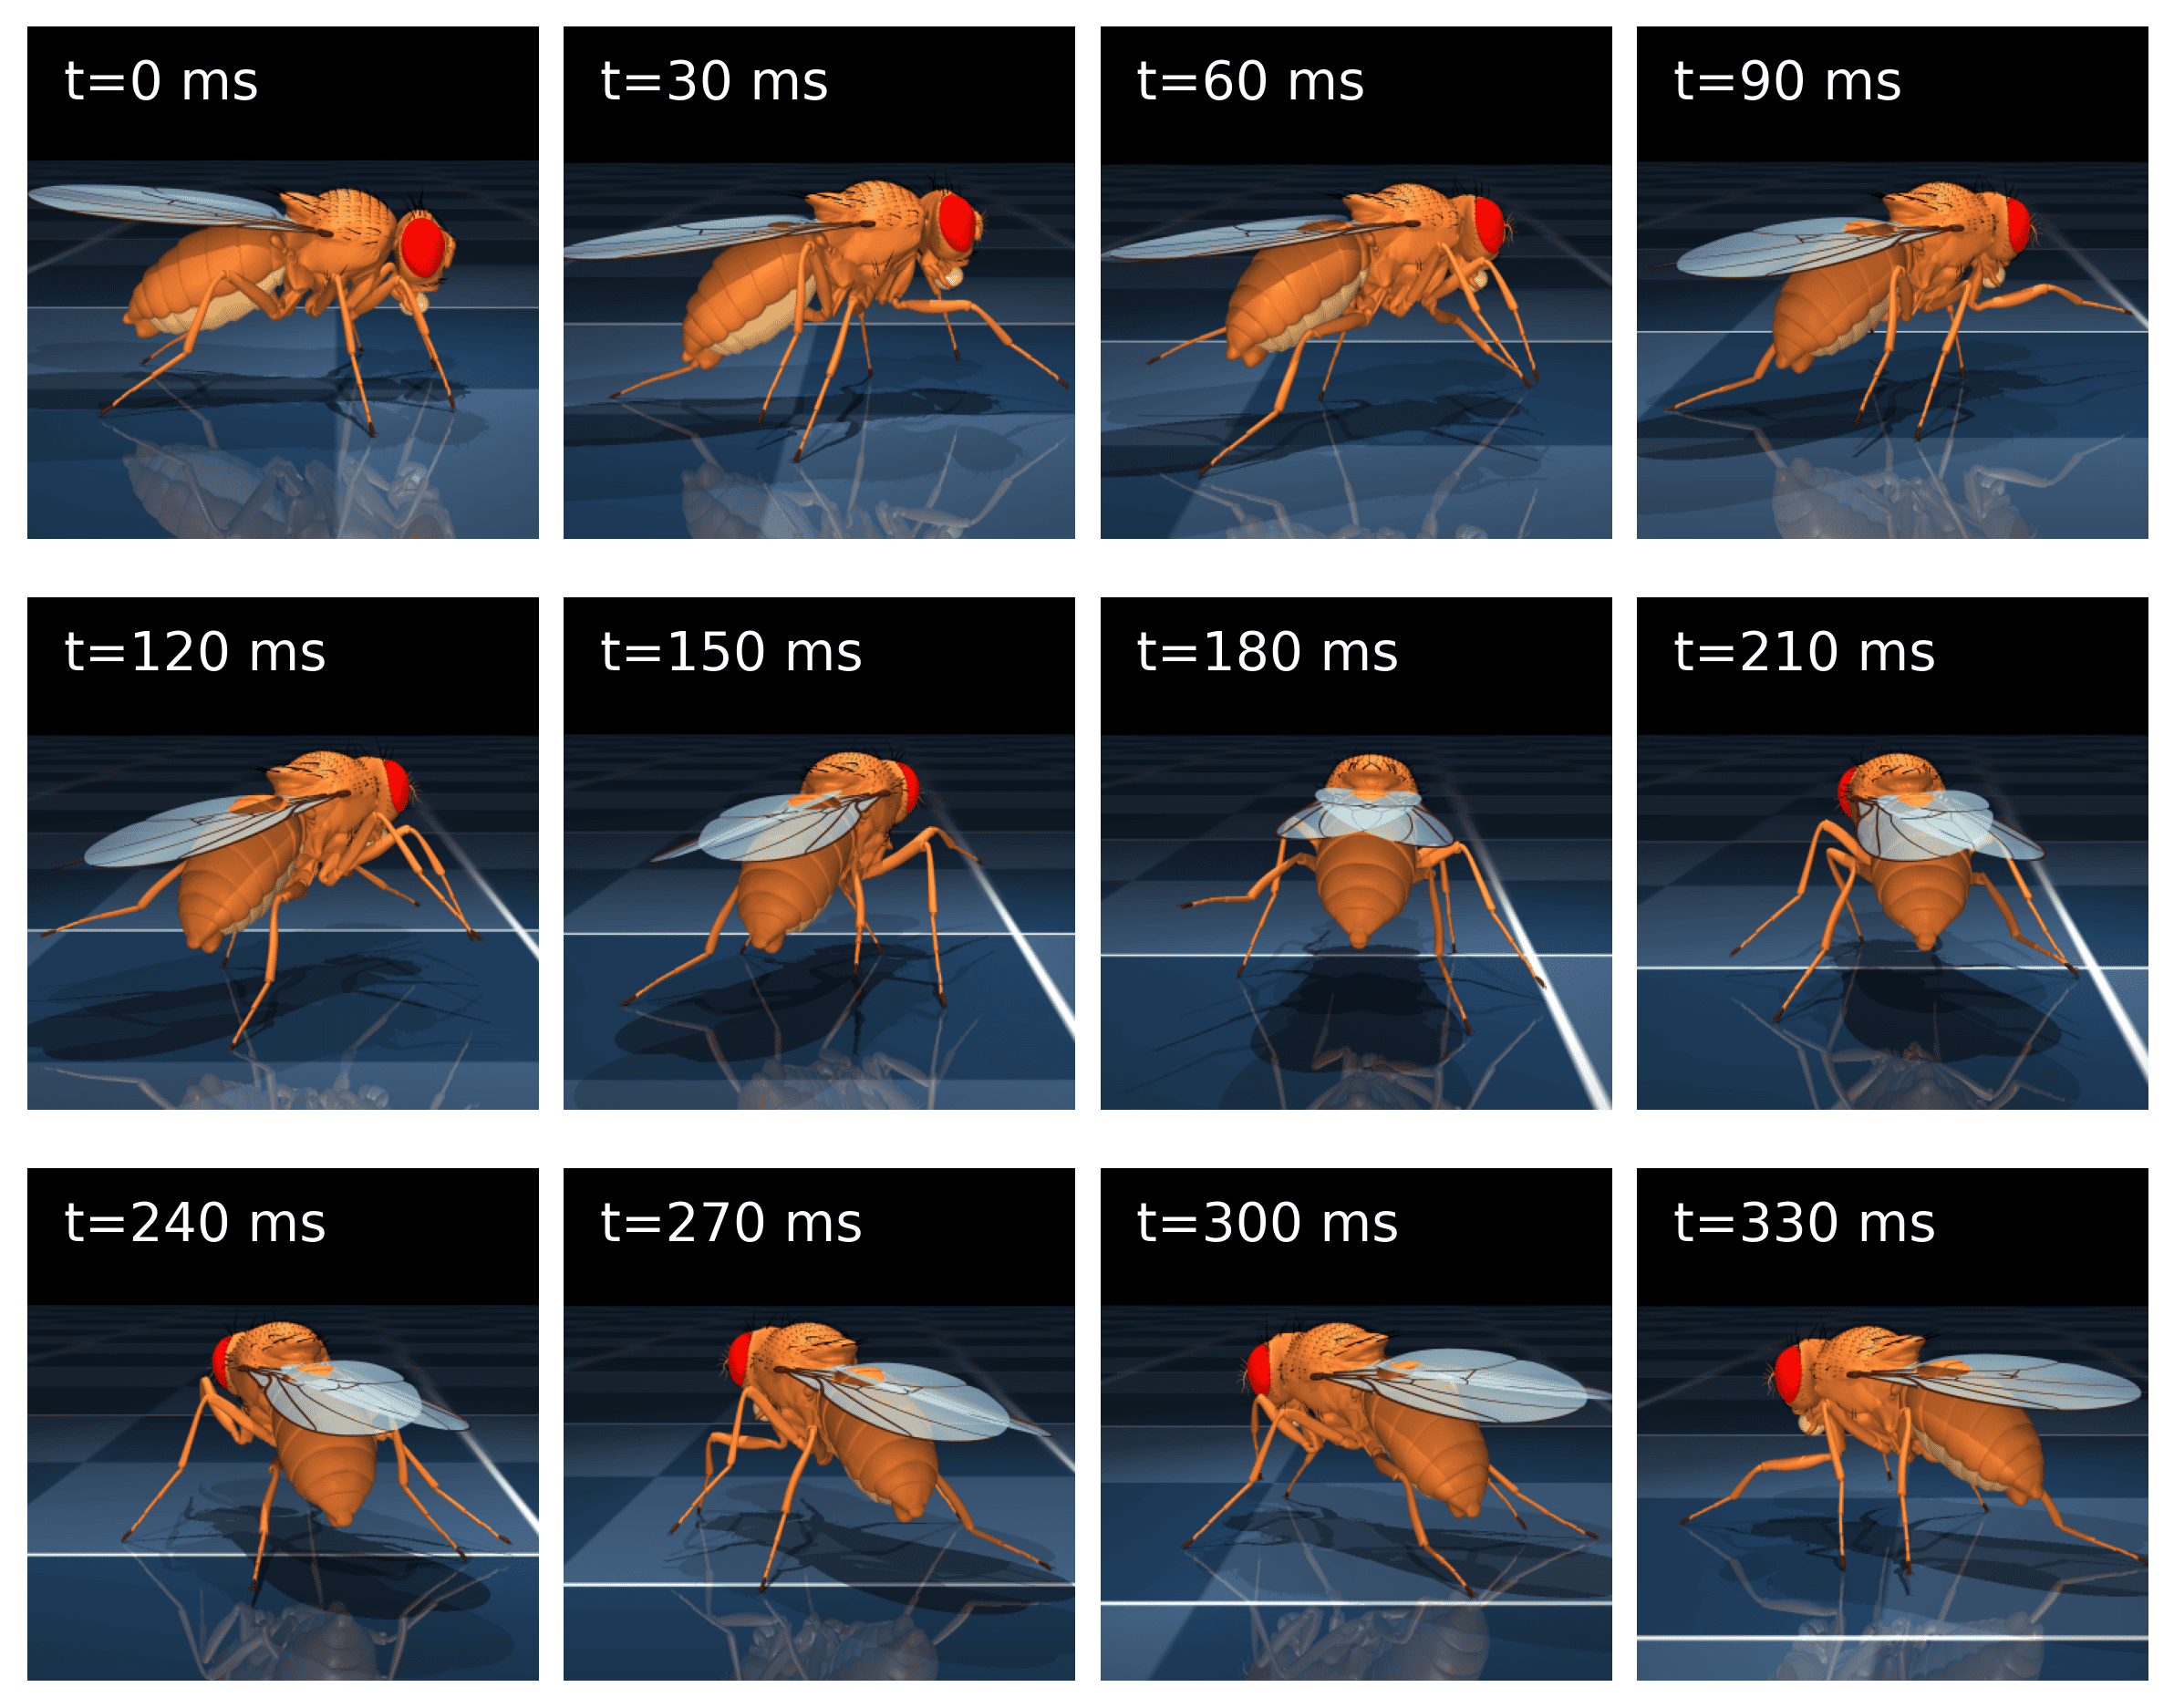
\includegraphics[width=0.395\textwidth]{figures/flyturn.png}
  \caption{\textbf{Turning dynamics.} Snapshots of the virtual fly executing a high-speed left turn at 3 cm/s and 10 rad/s.}
  \label{fig:flyturn}
\end{figure}

The ability to perform both straight walking and turning indicates that the learned FlyGM policy does not simply memorize a single stereotyped gait, but rather encodes a flexible control strategy that can adapt to new locomotor demands. These findings highlight the robustness of the architecture and suggest its potential for modeling a wider repertoire of multi-task behaviors.

\textbf{Flight}

\label{sec:fly_task}

To assess whether FlyGM can generalize beyond terrestrial locomotion, we additionally trained the fly to perform a flying task. In this setting, the policy served as a higher-level neural controller that modulated the output of the wing-beat pattern generator, thereby enabling stable flight dynamics.

\begin{figure}[htbp]
  \centering
  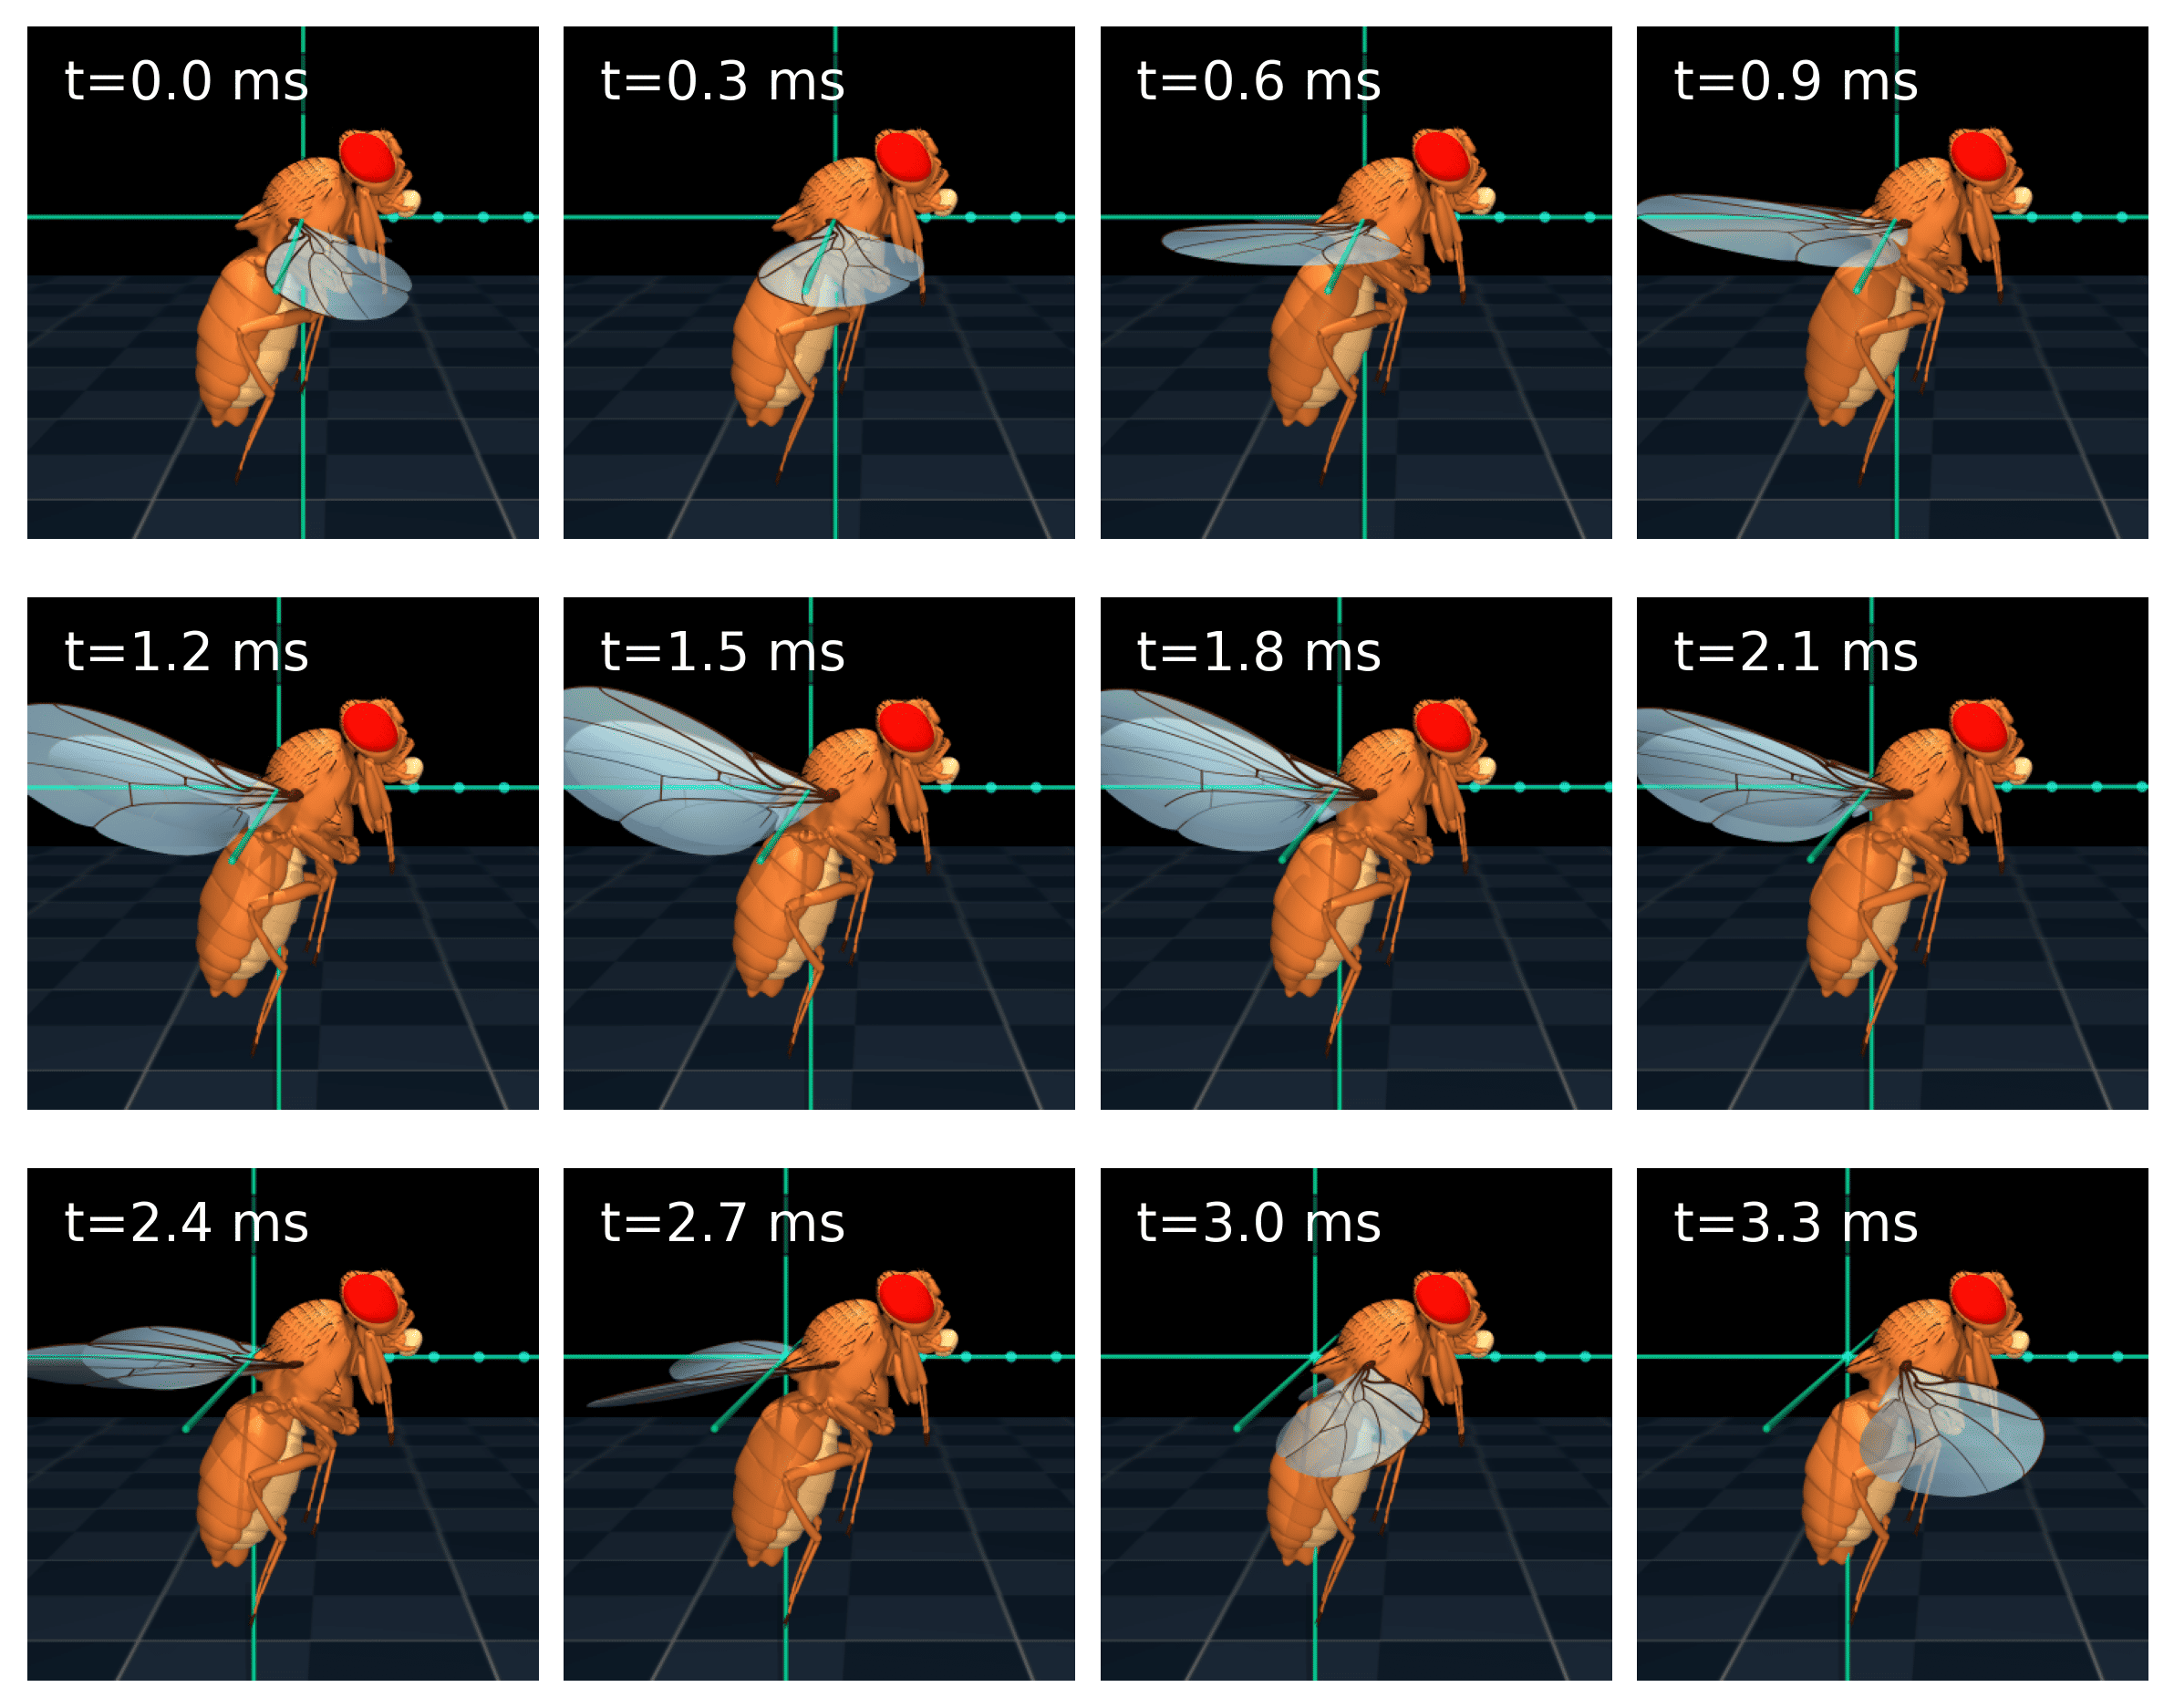
\includegraphics[width=0.395\textwidth]{figures/flyflight.png}
  \caption{\textbf{Flight dynamics.} Snapshots of the virtual fly executing a straight flight task at a velocity of 20 cm/s.}
  \label{fig:flyflight}
\end{figure}

As shown in Figure~\ref{fig:flyflight}, the trained controller maintained stable forward flight at a constant speed and kept body orientation aligned with the target direction, demonstrating that the connectome-based network can extend from walking to flight locomotion.

These results suggest that connectome-structured networks are not limited to walking but can support a broader repertoire of multimodal behaviors, highlighting the generality of this modeling framework for embodied control.

\subsection{Neural Representations Analysis}

\begin{figure*}[t]
  \centering
  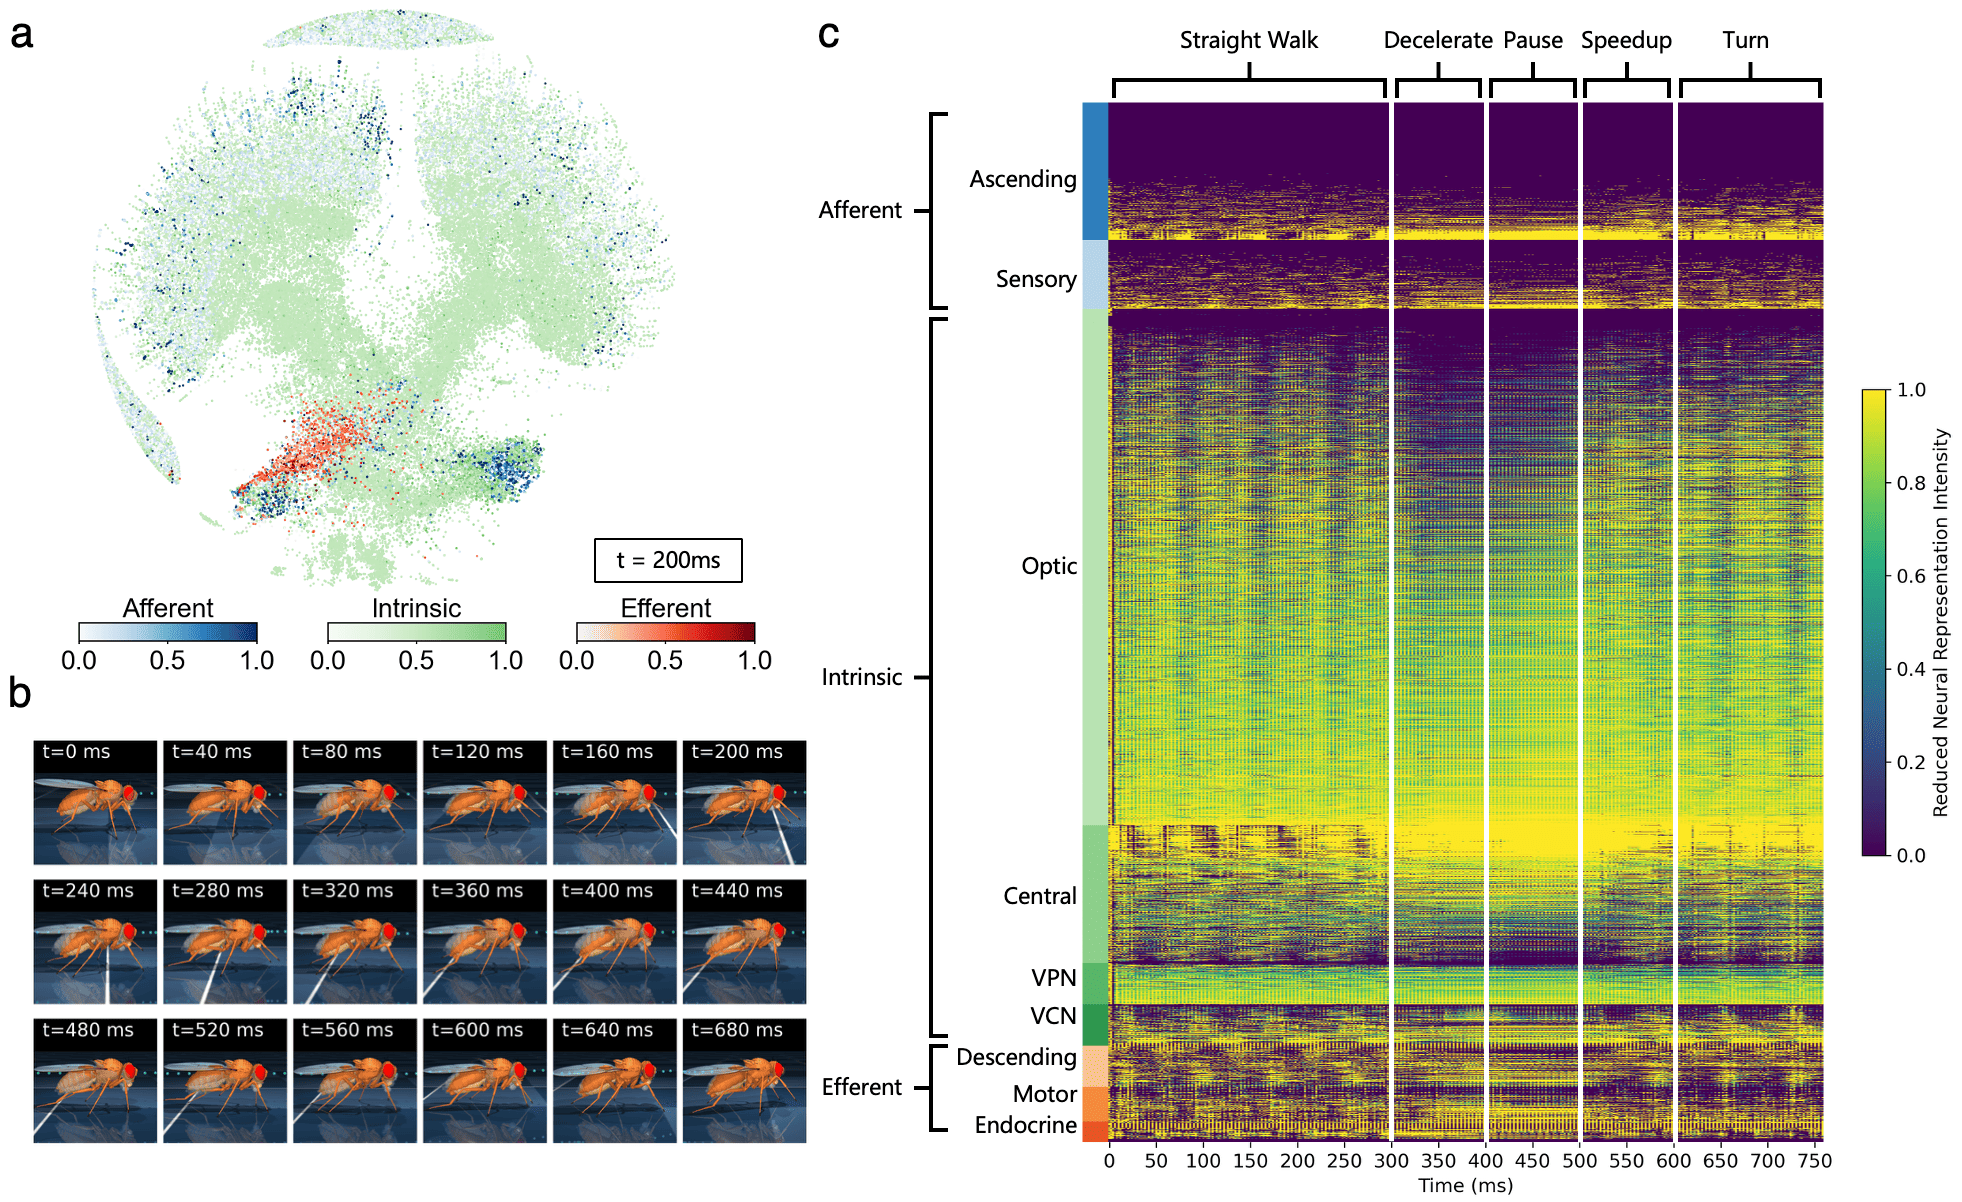
\includegraphics[width=0.9\textwidth]{figures/repr_v2.png}
  \caption{\textbf{Neural and behavioral dynamics across a continuous walking sequence.} 
  \textbf{(a)} Force-directed layout of the connectome at 200 ms, with neurons colored by flow type and representation intensity.
  \textbf{(b)} Behavioral snapshots (0–680 ms) show straight walking, decelerating, pausing, speeding-up, and turning phases; blue dots and ghost fly mark target trajectory and orientation.
  \textbf{(c)} Temporal dynamics across the connectome, grouped by flow type and major neuron classes and showing transitions between behavioral phases.
  }
  \label{fig:repr_v2}
\end{figure*}

Connectome-based architectures provide a unique opportunity to study how information propagates through biological wiring. By recording neuron states during simulation, we used the \textbf{reduced neural representation intensity} as an indicator of neural activity. High-dimensional features ($\mathcal{T} \times \mathcal{N} \times \mathcal{C}$, $\mathcal{T}$ for time steps, $\mathcal{N}$ for neuron counts, and $\mathcal{C}$ for channel dimension) were compressed into a single-channel signal via Principal Component Analysis (PCA) along the channel dimension. The resulting values were then clipped to the 5th–95th percentile range and min-max normalized to $[0,1]$ to improve comparability and reduce outlier effects. This metric serves as a scalar proxy for the engagement level of individual neurons, allowing us to map complex, multi-channel latent dynamics onto a single-intensity scale that facilitates the visualization of population-level information flow.

Figure~\ref{fig:repr_v2} presents the temporal dynamics of reduced neural representation intensity in a long composite locomotion sequence. Figure~\ref{fig:repr_v2}a visualizes the connectome at 200 ms using a force-directed layout that spatially arranges neurons based on their connectivity. Neurons are colored by flow type and shaded by representation intensity, illustrating the spatial distribution of the reduced neural representation intensity within the connectome-structured space at a specific moment. Therefore, we can observe the activation patterns of neurons of different flow types.

Figure~\ref{fig:repr_v2}c shows the temporal dynamics of neural representations across the connectome. Due to the extreme imbalance in superclass sizes (e.g., $>77000$ neurons in optic classes versus only 106 in motor classes), we employed stratified random downsampling to ensure visibility across all functional groups while preserving relative proportions (Detailed downsampling setting see Appendix~\ref{app:Dawnsampling}). This approach maintained the diversity of neural responses while creating visually interpretable group representations.

To optimize the visualization of these dynamics, we reordered neurons within their functional classes using spectral sequencing. We first built the similarity matrix $S$ as follows:

\begin{equation}
S_{ij} = \alpha \text{sim}_{\text{cos}}(x_i, x_j) + (1 - \alpha)d_{ij}
\end{equation}

where $\text{sim}_{\text{cos}}$ is the cosine similarity, $d_{ij}$ is the normalized Euclidean distance, and $\alpha$ is set to 0.7.

We then constructed the symmetric normalized Laplacian matrix:
\begin{equation}
L = I - D^{-1/2} S D^{-1/2}
\end{equation}
where $D$ is the degree matrix with $D_{ii} = \sum_j S_{ij}$. Eigendecomposition of $L$ was performed to obtain its eigenvalues $\lambda_0 \le \lambda_1 \le \dots \le \lambda_n$ and corresponding eigenvectors $\mathbf{v}_0, \mathbf{v}_1, \dots, \mathbf{v}_n$. The optimal ordering was determined by the Fiedler vector $\mathbf{v}_1$, which was the eigenvector corresponding to the second smallest eigenvalue $\lambda_1$. The final visualization sequence was obtained by:
\begin{equation}
\pi = \text{argsort}(\mathbf{v}_1)
\end{equation}
This reordering ensures that neurons with similar temporal activation patterns are positioned adjacently, revealing the emergent functional specialization across superclasses.

The resulting plots demonstrate heterogeneous responses to phase transitions across different neuron superclasses, whereas neurons within the same superclass display relatively consistent response patterns. Distinct activation patterns emerge for each class, and transitions between behavioral phases imply how sensory observations and motor intentions are dynamically transmitted through the network. Such patterns are consistent with experimental neuroscience findings~\citep{Brezovec2024,schaffer2023spatial}. These results show the potential to align FlyGM dynamics with neurophysiological processes.

\section{Conclusion and Discussion}

Without neural architecture search or optimization, this work demonstrates that the whole-brain connectome-based graph model FlyGM can serve as an efficient reinforcement learning controller to achieve diverse movement tasks of a simulated biomechanical fruit fly. By structuring information flow according to the FlyWire connectome, FlyGM replaces hand-crafted policy networks with a graph-based network that directly reflect the wiring diagram of the brain.

Our results demonstrate that structural priors at the connectome scale provide a powerful inductive bias for embodied control. Even when simplified to an unweighted directed graph without synapse counts or neurotransmitter types, the connectome is sufficient to drive diverse high-dimensional motor control. This suggests that wiring diagrams, long viewed as static anatomical maps, can be directly instantiated as functional networks for closed-loop control.

From the perspective of machine learning, FlyGM offers an anchor point for neural architecture search. Instead of relying on existing artificial structures, we can adapt structures from evolved biological networks. This provides a systematic alternative to generic architectures, potentially improving data efficiency, stability, and generalizability across tasks. The approach also opens the possibility of scaling to larger connectomes and more complex embodied agents, where the inductive biases of real nervous systems may be particularly advantageous.

Several limitations highlight opportunities for future progress. First, more detailed and complete connectome could be implemented to improve our model. Incorporating richer information may improve biological fidelity. Second, compared to MLP-based controllers, our model requires longer per-step computation and higher memory usage. Finally, extending the framework beyond locomotion will provide a more comprehensive test of the generality of connectome-based control.

In summary, FlyGM transforms static whole-brain connectomes into a dynamic model that can be used for whole-body motor control. By grounding policy architectures in biological wiring diagrams, this approach suggests a possibility towards more nature-aligned AI systems, and provides a computational platform for understanding sensorimotor transformation.

\newpage


\section*{Accessibility}

Project website is available at: \url{https://lnsgroup.cc/research/FlyGM}. This webpage provides supplementary materials, including demonstration videos of FlyGM across all evaluated locomotion tasks and the source code of FlyGM.

\section*{Software and Data}

To support the reproducibility of this work, we provide the complete codebase and data in an anonymous repository, accessible via the link provided on our project website: \url{https://lnsgroup.cc/research/FlyGM}. The implementation is based on PyTorch and PyTorch Geometric, integrating the FlyWire connectome dataset with the flybody MuJoCo physics simulation. All experimental configurations are included in the repository.

\section*{Impact Statement}

This work advances the field of Machine Learning by integrating biological connectomics with embodied control. This computational framework offers a potential means to simulate neural circuits in simulation, which may contribute to reducing animal usage in research. We believe there are no specific negative societal consequences or ethical risks that must be highlighted for this fundamental study.

\newpage
\bibliography{refs}
\bibliographystyle{icml2026}

\newpage
\appendix
\onecolumn

\section{Details of Model Architecture and Training Process}
\label{app:train_details}

\subsection{Model Architecture and Implementation}

The FlyGM model instantiates the Drosophila connectome as a large-scale recurrent neural system: synapse weights define a sparse linear aggregation operator, and each neuron additionally carries trainable intrinsic parameters that condition how synaptic input updates its state. The network is structured as a directed graph where nodes represent neurons and edges represent synaptic connections, partitioned into afferent, intrinsic, and efferent sets based on information flow. The model processes inputs through the following components:

Input Normalization: A RunningNorm layer is applied to observations to stabilize training by maintaining running estimates of mean and variance. This layer operates online and is updated during training.  

Encoder: Observations are projected into the afferent neuron state space via a linear layer followed by ReLU activation.  

Graph Propagation: Information is propagated through the connectome using a message-passing mechanism with gated updates combining previous states and incoming messages.  

Decoder: Efferent neuron states are aggregated and passed through a multi-layer perceptron with ReLU activations, outputting action means and standard deviations via linear and softplus heads, respectively.  

All experiments were conducted on servers equipped with NVIDIA A100 80GB PCIe GPUs and Intel Xeon Gold 6348 CPUs.

\subsection{Training Pipeline}

Training proceeds in two stages:  

Imitation Learning: The policy is initialized by mimicking expert trajectories generated by a pre-trained MLP controller provided by flybody. This stage uses PyTorch Lightning for distributed training across multiple workers.  

Reinforcement Learning: The model is fine-tuned with Proximal Policy Optimization to maximize task rewards. This stage is implemented using PyTorch Distributed Data Parallel (DDP) for scalability.  

Optimization uses AdamW with a learning rate scheduler (ReduceLROnPlateau) that reduces the learning rate upon validation loss improving. Both stages employ gradient clipping to ensure stability.

\subsection{Task-Specific Configurations}
Walking Task:
\begin{itemize}
\setlength{\itemsep}{0pt}
\setlength{\parsep}{0pt}
\setlength{\parskip}{0pt}
    \item Observation dimension: 1,253 (proprioceptive + exteroceptive + visual inputs),
    \item Action dimension: 59 (joint actuators and adhesion controls),  
    \item Learning rate: $1 \times 10^{-4}$,  
    \item Message-Passing: 32 node channels, 4 message-passing layers,
    \item Expert policy architecture: 512–512–512–512 fully-connected layers with LayerNorm + Tanh (first layer) and ELU activations, outputting mean (Linear) and std (Linear + Softplus) for 59-dimensional actions.
\end{itemize}

Flight Task:
\begin{itemize}
\setlength{\itemsep}{0pt}
\setlength{\parsep}{0pt}
\setlength{\parskip}{0pt}
    \item Observation dimension: 104 (simplified proprioceptive and kinematic inputs), 
    \item Action dimension: 12 (wing torques, pattern generator modulation, body joints), 
    \item Learning rate: $1 \times 10^{-5}$,
    \item Message-Passing: 32 node channels, 4 message-passing layers,  
    \item Expert policy architecture:  256–256–256 fully-connected layers with LayerNorm + Tanh (first layer) and ELU activations, outputting mean (Linear) and std (Linear + Softplus) for 12-dimensional actions.
\end{itemize}

Both tasks use identical graph topology derived from the FlyWire connectome but differ in input/output dimensions and network hyperparameters due to behavioral constraints. Training metrics are logged for performance monitoring.

\section{Detailed Settings of Locomotion Environment}
\label{app:env_details}

Our experiments follow the locomotor task design introduced in the flybody simulator, which provides imitation-learning datasets for terrestrial (\emph{walking}) and aerial (\emph{flight}) behaviors. 

We evaluate four tasks: 
\begin{itemize}
\setlength{\itemsep}{0pt}
\setlength{\parsep}{0pt}
\setlength{\parskip}{0pt}
    \item Gait initiation: generating stable stepping patterns from rest, 
    \item Straight-line walking: tracking forward centre-of-mass (CoM) trajectories, 
    \item Turning: executing lateral turns at constant speed, 
    \item Flight: stabilizing and steering free flight trajectories.
\end{itemize}
For walking-based tasks, the default setting of flybody receives a 741-dimensional proprioceptive/exteroceptive observation, comprising:
\begin{itemize}
\setlength{\itemsep}{0pt}
\setlength{\parsep}{0pt}
\setlength{\parskip}{0pt}
  \item accelerometer (3), gyro (3), velocimeter (3), world $z$-axis (3),
  \item actuator activations (59),
  \item appendage pose (21), force sensors (18),
  \item joint positions (85) and velocities (85),
  \item tactile contacts (6),
  \item reference displacement (195) and root quaternion (260).
\end{itemize}
We augment this with binocular visual input: left and right eye cameras ($32\times32\times3$ RGB each) downsampled and resized to two $16\times16$ grayscale figures. The final observation dimension is 1,253.  

Actions remain 59-dimensional, actuating adhesion, head/abdomen motion, and all leg joints as in default settings of flybody walking task.

For the flight task, we keep the flybody sensory design with a 104-dimensional input comprising:
\begin{itemize}
\setlength{\itemsep}{0pt}
\setlength{\parsep}{0pt}
\setlength{\parskip}{0pt}
    \item accelerometer (3), gyro (3), velocimeter (3), world $z$-axis (3),
    \item joint positions (25) and velocities (25),
    \item reference displacement (18) and root quaternion (24).
\end{itemize}
The policy outputs 12 control signals: instantaneous wing torques, head/abdomen angles, and Wing-Pattern Generator (WPG) frequency modulation. The WPG provides a nominal wing-beat template, while the policy learns residual corrections.

\section{Joint kinematics and actuator activations during walking}
\label{app:kinematics}

To further investigate the motor control strategy learned by FlyGM, we analyze the joint-level kinematics and corresponding actuator activations during stable walking. As illustrated in Figure~\ref{fig:coxa}, the model exhibits rhythmic coxa joint oscillations that are tightly coupled with the underlying actuator drive. Specifically, the temporal profiles of both joint angles and activations reveal a clear alternating tripod gait: the left T1/T3 and right T2 legs form one functional group, while the right T1/T3 and left T2 legs form the other. These two groups operate in anti-phase, maintaining the static stability required for hexapedal locomotion. The synchronization between descending control signals (actuator activations) and the resulting physical movement (joint angles) demonstrates that the connectome-structured policy effectively translates brain-wide message passing into coordinated whole-body movement, consistent with the kinematic patterns observed in biological Drosophila.

\begin{figure*}[htbp]
  \centering
  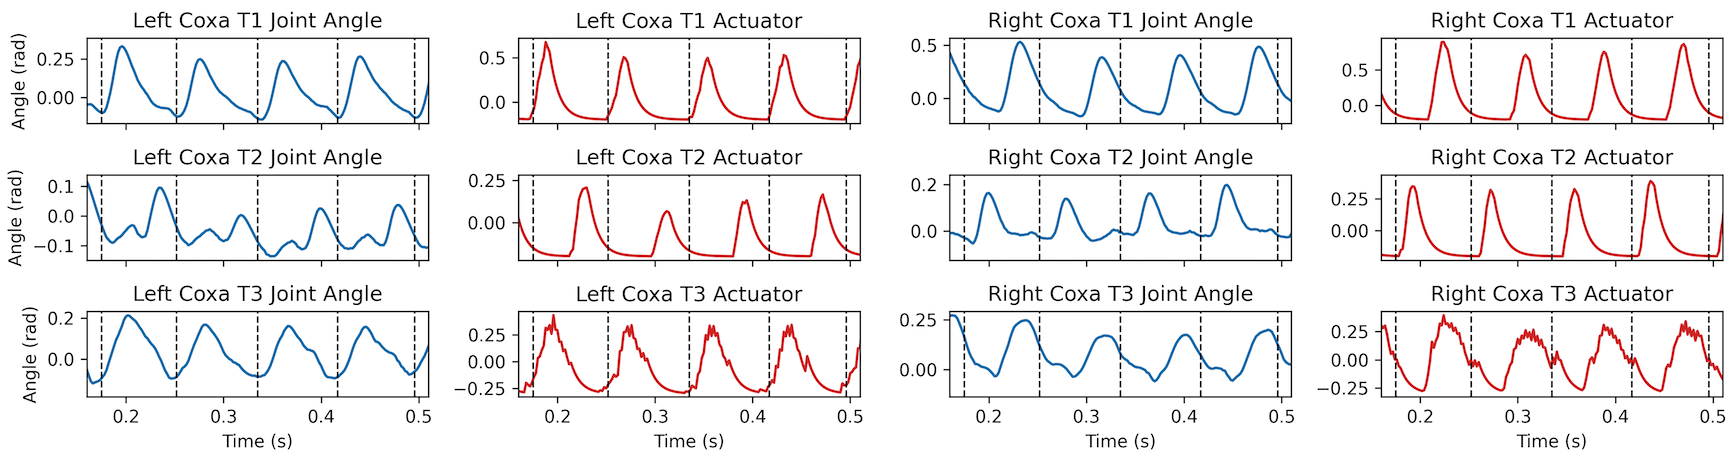
\includegraphics[width=1\textwidth]{figures/coxa.png}
  \caption{\textbf{Joint kinematics and actuator activations during walking.} 
  We visualize the angles (blue) and actuator activations (red) of coxa joints from left (T1–T3) and right (T1–T3) legs over multiple gait cycles. Dashed vertical lines mark gait phases based on the troughs of the left T1 coxa. The model reproduces alternating tripod-like coordination, with left T1/T3 synchronized with right T2, and left T2 synchronized with right T1/T3, consistent with expected fly walking patterns.}
  \label{fig:coxa}
\end{figure*}

\section{Detailed Method for Visualization}

\subsection{Figure 2(a)}

We visualized the aggregated synapse graph of the fly connectome using the FlyWire FAFB v783 dataset, with nodes classified by superclass labels provided by FlyWire. The node size reflects the number of neurons in each class, while the thickness and darkness of the directed edges represent the number of aggregated synaptic connections.

\subsection{Figure 2(b)}

In the visualization of the network of connectome, we did not incorporate the three-dimensional structural priors of Drosophila neurons. Instead, we employed a force-directed layout algorithm~\citep{Kobourov2012} for graph drawing. In this method, edges are modeled as springs while nodes exert repulsive forces on each other, and the system iteratively evolves toward a low-energy equilibrium. This layout highlights the topological organization of the network, making the relationships among different super-classes and subgroups more visually apparent. For visualization, we applied a threshold of more than 25 synapses and retained only connections exceeding this cutoff.

\subsection{Downsampling in Figure 8(c)}
\label{app:Dawnsampling}

The downsampling thresholds were set as follows: sensory: 400, ascending: 200, optic: 1500, central: 400, visual projection: 120, visual centrifugal: 120, descending: 120, motor: 100, endocrine: 60. This approach maintained the diversity of neural responses while creating visually interpretable group representations.

\end{document}